\documentclass[a4paper,11pt]{article}

% Package imports
\usepackage{amsmath, amssymb, amsthm}
\usepackage{mathtools}
\usepackage{stmaryrd}
\usepackage{graphicx}
\usepackage{fancyhdr}
\usepackage{geometry}
\usepackage{setspace}
\usepackage{titlesec}
\usepackage{chngcntr}
\usepackage{booktabs}
\usepackage{listings}
\usepackage{enumitem}
\usepackage{caption}
\usepackage{subcaption}
\usepackage{framed}
\usepackage{bm}
\usepackage[nolist]{acronym}
\usepackage[most]{tcolorbox}
\usepackage{tikz}
\usepackage{needspace}

% Page layout
\geometry{left=2cm, right=2cm, top=2.5cm, bottom=2.5cm}
\graphicspath{ {./images/} }

% List definition
\setlist[itemize]{leftmargin=7.5mm}
\setlist[enumerate]{leftmargin=7.5mm}
% \setlist[itemize,2]{label=$\circ$}

% Header definition
\pagestyle{fancy}
\fancyhf{}
\lhead{Quantencomputer Skript (Dr. Thomas Wellens)}
\rhead{\thepage}


% Custom commands for numbered definitions
\newcounter{definitioncounter}
\counterwithin{definitioncounter}{section}
\newtcolorbox{definitionbox}[2][]{
  enhanced,
  colback=white,
  colframe=black,
  coltitle=black,
  boxrule=.5pt,
  arc=5pt,
  fonttitle=\bfseries,
%   title filled=true,
  title={Definition \thedefinitioncounter\hspace{.8em}(#2)},
%   title=My Title,
  attach boxed title to top left={yshift=-0.7\baselineskip-0.4pt,xshift=3mm},
  boxed title style={
    colback=white,
    colframe=white,
    left=6pt,
    right=6pt,
    % before upper=\strut
  },
%   boxed title style={tile,size=minimal,left=0.5mm,right=0.5mm, colback=white,before upper=\strut}
  top=15pt,
  bottom=10pt,
  left=6pt,
  right=6pt,
  #1
}

\setlength{\parindent}{0pt}
\setlength{\skip\footins}{0.5cm} % Adjust this to change the space above the footnotes
\raggedbottom


% CUSTOM MACROS
\newcommand{\definition}[2]{
    \vspace{.05cm}
    \refstepcounter{definitioncounter}
    \begin{definitionbox}{#1}
    #2
    \end{definitionbox}
}

\newcommand{\ig}[2]{ % includegraphics
  \includegraphics[width=#1\textwidth]{#2}
}
\newcommand{\cig}[2]{  % includegraphics (centered)
  \begin{center}
    \includegraphics[width=#1\textwidth]{#2}
  \end{center}
}

\newcommand{\cf}[1]{\[#1\]} % centered formula
\newcommand{\f}[1]{${#1}$} % inline formula
\renewcommand{\b}[1]{\textbf{#1}} % bold text
\renewcommand{\it}[1]{\textit{#1}} % italic text

% QC symbol macros for use in text
\newcommand{\ket}[1]{\f{|#1\rangle}} % ket
\newcommand{\bra}[1]{\f{\langle#1|}} % bra

% QC symbol macros for use !inside! of formulas
\newcommand{\cket}[1]{|#1\rangle} % ket
\newcommand{\cbra}[1]{\langle#1|} % bra
\newcommand{\skal}[2]{\left\langle#1|#2\right\rangle} % scalar product: <a|b> 
\newcommand{\matr}[1]{\begin{pmatrix}#1\end{pmatrix}} % matrix shortcut
\newcommand{\tr}[1]{\text{Tr}(#1)} % trace

\begin{document}

% Title section
\begin{center}
    {\huge Quantencomputer Skript - WS25/26\par}
    \vspace{0.5cm}
    {\large Niklas Rodenbüsch \par}
    \vspace{0.5cm}
    {\large \today \par}
\end{center}
\vspace{0.5cm}



\onehalfspacing
\captionsetup{justification=centering}

\section{Vorlesung}
\subsection{Quantencomputer}
\definition{Quantencomputer}{
        Quantencomputer funktionieren nach quantenmechanischen Gesetzen und haben das Potential, bestimmte (aber nicht alle) Rechenaufgaben effizienter als klassische Computer zu lösen.\\
        Die heutigen (10.2025) Quantencomputer sind jedoch noch zu klein und zu fehlerbehaftet, um den klassischen überlegen zu sein. Dieser Punkt könnte jedoch irgendwann in den nächsten Jahren erreicht werden.
}
\subsection{Aufbau der Vorlesung}
Diese Vorlesung vermittelt einen Einblick in die zugrunde liegenden quantenmechanischen Gesetze, die allgemeine Funktionsweise eines Quantencomputers, und stellt für mögliche Anwendungen geeignete \b{Quantenalgorithmen} vor:
\begin{itemize}
    \item \b{Shor-Algorithmus} zur Faktorisierung großer Zahlen
    \item \b{Grover-Algorithmus} zum Auffinden eines gesuchten Elements in einer unstrukturierten Menge
    \item \b{HHL-Algorithmus} zur Lösung linearer Gleichungssysteme
    \item \b{\ac{vqe}} zur Bestimmung der Grundzustandsenergien von Molekülen (wichtig zur Berechnung chemischer Reaktionszeiten)
    \item \b{\ac{qaoa}} zur Lösung von Optimierungs- problemen (z.B. in der Finanzmathematik oder Logistik)
\end{itemize}
\section{Besonderheiten von Quantencomputern}
\textbf{Klassische Computer} funktionieren mit Bits (0 oder 1). Der Zustand eines klassischen Computers (genauer gesagt: seines Arbeitsspeichers) kann zu jedem Zeitpunkt durch eine Reihe von Nullen oder Einsen beschrieben werden, z.B.:
\cf{0\ 0\ 1\ 0\ 1\ 0\ 1\ 1\ 1\ 0\ 0\ 1\ 1\ 1\ 0\ 0\ 0\ 0\ 1\ \dots} 
\textbf{Quantencomputer} funktionieren mit \b{Qubits}. Ein solches Qubit hat auch zwei mögliche Zustände, die mit \ket{0} und \ket{1} bezeichnet werden. Dies können z.B. verschiedene elektronische Zustände eines Atoms sein:

\begin{figure}[h!]
    \centering
    
\includegraphics[width=.4\textwidth]{images/bahnen.png}
    \caption{In der QM gibt es eigentlich keine "Bahnen"! Gezeigt werden soll: Im Zustand \ket{0} bzw. \ket{1} hält sich das Elektron mit unterschiedlichen Wahrscheinlichkeiten an verschiedenen Orten auf.}
\end{figure}

Nach den Gesetzen der \ac{qm} sind jedoch auch Überlagerungen ("Superpositionen") dieser beiden Zustände möglich:
\cf{
    \cket{\psi} = a_0\cket{0}+a_1\cket{1}\quad\textrm{, wobei } a_0,a_1\in\mathbb{C} 
}
Das Qubit befindet sich dann gewissermaßen "gleichzeitig" in Zustand \ket{0} und \ket{1}. Versucht man, durch Messung, den Zustand auszulesen, so ist es allgemein unmöglich, das Ergebnis der Messung mit Sicherheit vorherzusagen: Man findet entweder das Ergebnis "\ket{0}" (mit Wahrscheinlichkeit \f{|a_0|^2}), oder "\ket{1}" (mit Wahrscheinlichkeit \f{|a_1|^2}). Daher muss gelten: \f{|a_0|^2+|a_1|^2=1}\\

Zustände mehrerer Qubits haben entsprechend folgende Form:
\begin{align*}
    \text{2 Qubits: }\cket{\psi} =\ & a_{00}\cket{00}+a_{01}\cket{01}+a_{10}\cket{10}+a_{11}\cket{11}\quad&\Rightarrow\ &4=2^2\text{ komplexe Zahlen nötig,}\\
    &&& \text{ um Zustand zu beschreiben}\\
    \text{3 Qubits: }\cket{\psi} =\ & a_{000}\cket{000}+a_{001}\cket{001}+a_{010}\cket{010}+a_{011}\cket{011}+&\\
    &a_{100}\cket{100}+a_{101}\cket{101}+a_{110}\cket{110}+a_{111}\cket{111}\quad&\Rightarrow\ &2^3 = 8\\
    \text{n Qubits: }\cket{\psi} =\ & a_{00\dots00}\cket{00\dots00}+a_{00\dots01}\cket{00\dots01}+\dots &\Rightarrow\ & 2^n
\end{align*}
Für großes \f{n} ist es daher unmöglich, einen Quantencomputer auf einem klassischen Computer zu simulieren, da der Speicher nicht ausreicht, um alle Koeffizienten \f{a_{00\dots00}, a_{00\dots01}, \dots} zu speichern. In der Praxis ist dieser Punkt zur Zeit bei \f{n\approx 60} erreicht, theoretisch spätestens bei \f{n=160}, da \f{2^{160} \approx 10^{48}} ungefähr \f{\frac{1}{10}} der Anzahl der Atome in der Erde entspricht.\\

\b{Aber:} Eine Überlagerung von \f{2^n} Zuständen an sich ist nicht hilfreich, da beim Auslesen zum Schluss nur einer dieser Zustände als Ergebnis auftritt (z.B. Ergebnis "\f{00\dots00}" mit Wahrscheinlichkeit \f{|a_{00\dots00}|^2}). Quantenalgorithmen müssen also so konstruiert werden, dass nur die gewünschten Ergebnisse (d.h. die Lösungen des gegebenen Problems) mit hoher Wahrscheinlichkeit auftreten. Dies ist schwierig, und bislang gibt es nur für einige spezielle Probleme geeignete Algorithmen.\\

\b{Außerdem:} Quantenmechanische Überlagerungen sind sehr empfindlich gegenüber Störungen. Die Qubits müssen extrem gut von ihrer Umgebung isoliert werden, was in der Praxis schwierig zu be- werkstelligen ist.

\section{Quantenmechanische Grundlagen}
\subsection{Lineare Algebra}
\definition{Vektorraum}{
    Vektoren eines \f{N}-dimensionalen komplexen Vektorraums \f{V} mit Basis \f{B = (v_1, v_2, \dots, v_n)} haben folgende Form:
    \cf{
        v = a_1v_1+a_2v_2+\dots+a_Nv_N = \begin{pmatrix}
            a_1\\a_2\\\vdots\\a_N
        \end{pmatrix} \quad\leftarrow\quad \begin{matrix}
            \text{(Darstellung des Vektors }v\\\text{bzgl. Basis }v_1, v_2, \dots, v_N)
        \end{matrix}
    }
    \b{Addition \& Skalarmultiplikation: }
    \cf{
        \begin{pmatrix}
            a_1\\a_2\\\vdots\\a_N
        \end{pmatrix} + \begin{pmatrix}
            b_1\\b_2\\\vdots\\b_N
        \end{pmatrix} = \begin{pmatrix}
            a_1+b_1\\a_2+b_2\\\vdots\\a_N+b_N
        \end{pmatrix} \quad;\quad
        \lambda\begin{pmatrix}
            a_1\\a_2\\\vdots\\a_N
        \end{pmatrix} = \begin{pmatrix}
            \lambda a_1\\\lambda a_2\\\vdots\\\lambda a_N
        \end{pmatrix} \quad;\quad a_1, \dots, a_N \in \mathbb{C}
    }
}
\definition{Komplexe Konjugation}{
    Eine komplexe Zahl \f{z} kann wie folgt komplex konjugiert werden:
    \f{
        z = a + bi \mapsto z^* = \bar{z} = a - bi
    }
}
\definition{Lineare Operatoren (Matrizen)}{
    Ein linearer Operator \f{A} hat folgende Eigenschaften:
    \begin{gather*}
        A:V \mapsto Av\in V\\
        A(v+w) = Av+Aw\\
        A(\lambda v) = \lambda (Av)
    \end{gather*}
    \b{Matrizenmultiplikation:}
    \cf{
        (AB)v = A(Bv) \quad\implies\quad \text{bekannte Regel für Multiplikation zweier Matrizen}
    }
    \b{Adjungierter Operator:}
    \cf{
        \quad A^\dagger = (A^*)^\top = \begin{pmatrix}
            A_{11}^* & \dots & A_{N1}^* \\
            \vdots & \ddots & \vdots \\
            A_{1N}^* & \dots & A_{NN}^* 
        \end{pmatrix} \quad,\quad
        (AB)^\dagger = B^\dagger A^\dagger \quad,\quad
        (\lambda A)^\dagger = \lambda^*A^\dagger
    }
}
\definition{Besondere Operatoren}{
    \begin{itemize}
        \item Selbstadjungierter Operator: \f{A=A^\dagger}
        \item Unitärer Operator \f{U}: \f{UU^\dagger = U^\dagger U = \mathbb{I}}
        \item Projektor \f{P}: \f{P=P^\dagger} und \f{P^2=p}
    \end{itemize}
}
\definition{Skalarprodukt}{
    \cf{
        v = \begin{pmatrix}
            a_1 \\ \vdots \\ a_N
        \end{pmatrix}, w = \begin{pmatrix}
            b_1 \\ \vdots \\ b_N
        \end{pmatrix} \implies \left\langle v,w \right\rangle = v^\dagger w = (a_1^*,\dots,a_N^*)\begin{pmatrix}
            b_1\\ \vdots \\ b_N
        \end{pmatrix} = a_1^*b_1+\dots+a_N^*b_N
    }
    Es gelten folgende Rechenregeln:
    \begin{gather*}
        \left\langle u,v+w\right\rangle = \left\langle u,v\right\rangle + \left\langle u,w\right\rangle   \\
        \left\langle u, \lambda v\right\rangle = \lambda \left\langle u,v\right\rangle  \\
        \left\langle u,v\right\rangle = \left\langle v,u\right\rangle^*  \\
        \implies \left\langle u+v,w\right\rangle = \left\langle u,w\right\rangle + \left\langle v,w\right\rangle \quad,\quad \left\langle \lambda u,v\right\rangle = \lambda^*\left\langle u,v\right\rangle \quad,\quad \left\langle u,Av\right\rangle = \left\langle A^\dagger u,v\right\rangle   
    \end{gather*}
}
\definition{Weitere Begriffe}{
    \begin{itemize}
        \item \b{Norm:} \f{\left\lVert v\right\rVert \sqrt{\left\langle v,v\right\rangle } \geq 0 \quad (\left\lVert v\right\rVert = 0 \Leftrightarrow v = 0 )}
        \item \b{Orthonormalbasis:} \f{
            (v_1,\dots,v_N): \left\langle v_i,v_j\right\rangle = \delta_{ij} = \begin{cases}1 \text{ falls } i=j\\0 \text{ falls } i\neq j\end{cases} 
            }
        \item Für unitäre Matrizen U gilt: \f{\left\lVert Uv\right\rVert = \left\lVert v\right\rVert  }
    \end{itemize}    
}
\definition{Eigenwerte und Eigenvektoren}{
    \begin{itemize}
        \item \f{v} ist \ac{ev} von \f{A} mit \ac{ew} \f{\lambda \Leftrightarrow Av = \lambda v}
        \item Eine selbstadjungierte Matrix ist \b{unitär diagonalisierbar}, d.h. es gibt eine unitäre Matrix \f{U}, sodass \f{U^\dagger AU = \begin{pmatrix}
            \lambda_1 & & 0\\
            & \ddots & \\
            0 & & \lambda_N
        \end{pmatrix}}. \f{w_i = Uv_i} ist dann \ac{ev} von \f{A} mit \ac{ew} \f{\lambda_i \in \mathbb{R}}.
        \item Auch unitäre Matrizen sind unitär diagonalisierbar. Ihre \ac{ew} sind komplexe Zahlen mit Betrag \f{1}, d.h. \f{\lambda_k = e^{i\varphi_k}, \varphi_k\in\mathbb{R}}.
        \item Die \ac{ew} von \f{A} können durch Lösung folgender Gleichung berechnet werden: \f{\det(A-\lambda\mathbb{I}) = 0}
    \end{itemize}
}
\definition{Tensorprodukt}{
    Ist \f{\left\{v_i|i=1,\dots,N\right\} } eine Basis von \f{V} (dim\f{V=N}) und \f{\left\{w_i|i=1,\dots,M\right\} } eine Basis von \f{W} (dim\f{W=M}), so bildet \f{\left\{v_i\otimes w_j|i=1,\dots,N;j=1,\dots,M\right\}} eine Basis von \f{V\otimes W} mit dim\f{V\otimes W = NM}.    
    \b{Beispiel:}
    \cf{
        \left.\begin{array}{r}
            (v_1, v_2) \text{ Basis von }V\\
            (w_1,w_2,w_3)\text{ Basis von }W
        \end{array}\right\}\Rightarrow (v_1\otimes w_1, v_1\otimes w_2, v_1\otimes w_3, v_2\otimes w_1, v_2\otimes w_2, v_2\otimes w_3)
    }
    Für beliebige Vektoren \f{u,v\in V} und \f{w,x\in W} und \f{\lambda \in \mathbb{C}} gilt defintionsgemäß:
    \cf{
        \left.\begin{aligned}
            (\lambda v)\otimes w = v\otimes(\lambda w) = \lambda (v\otimes w) &\quad\\
            (u+v)\otimes w = u\otimes w + v\otimes w&\quad\\
            v\otimes (w+x) = v\otimes w + v\otimes x &\quad\\
    \end{aligned}\right\rvert \Rightarrow\quad
        v = \begin{pmatrix}
            a_1\\\vdots\\a_N
        \end{pmatrix},\quad
        w = \begin{pmatrix}
            b_1\\\vdots\\b_M
        \end{pmatrix}\quad v\otimes w = \begin{pmatrix}
            a_1b_1\\
            \dots\\
            a_1b_M\\
            a_2b_1\\
            \dots\\
            a_Nb_M
        \end{pmatrix}
    }
    \b{Verschränkung:}\\
    Falls ein Vektor \f{z\in V\otimes W} als ein Produkt zweier Vektoren \f{v\in V} und \f{w\in W} geschrieben werden kann (\f{z = v\otimes w}) so heißt \f{z} \b{Produktvektor}. Falls nicht, heißt \f{z} \b{verschränkt}.\\

    \b{Tensorprodukt von Operatoren:}\\
    Definiert als \f{(A\otimes B)(v\otimes w) := (Av)\otimes(Bw)}. Hieraus ergibt sich eine (naheliegende) Vorschrift zur Bestimmung der Matrixelemente von \f{A\otimes B}:
    \cf{
        A\otimes B = \begin{pmatrix}
            A_{11}B & \dots & A_{M1}B \\
            \vdots & \ddots & \vdots \\
            A_{1N}B & \dots & A_{MN}B
        \end{pmatrix}
    }
}

\subsection{Dirac-Notation von Vektoren in der Quantenmechanik}
In der Quantenmechanik werden Vektoren üblicherweise mit folgendem Symbol notiert:
\cf{
    \cket{v}\quad\text{("ket"-Vektor)}
}
Der adjungierte Vektor wird wie folgt geschrieben: \cf{\cket{v}^\dagger = \cbra{v}\quad\text{("bra"-Vektor)}}
Das Skalarprodukt zweier Vektoren \ket{v} und \ket{w} ergibt sich aus der Verschmelzung von \it{bra} und \it{ket} zu: 
    \cf{
    \left\langle v|w\right\rangle 
}
Zwischen \it{bra} und \it{ket} kann auch ein Operator stehen:
\cf{
    \left\langle v|A|w\right\rangle
}
Dies ist das Skalarprodukt von \ket{v} mit dem Vektor \f{A\cket{w}} bzw. das Skalarprodukt von \f{A^\dagger\cket{v}} mit \ket{w}: 
\cf{(A^\dagger\cket{v})^\dagger = \cket{v}^\dagger(A^\dagger)^\dagger = \cbra{v}A}
Neben dem Skalarprodukt gibt es auch ein "äußeres Produkt", bei dem \it{bra} und \it{ket} in umgekehrter Reihenfolge erscheinen:
\cf{
    \cket{v}\cbra{w}
}
Dies ist ein Operator, dessen Wirkung auf einen Vektor \ket{u} naheliegenderweise wie folgt definiert ist (wobei die runden Klammern weggelassen werden können):
\cf{
    (\cket{v}\cbra{w})\cket{u} = \cket{v}(\left\langle w|u\right\rangle) = \cket{v}\left\langle w|u\right\rangle
}
Von Mathematikern wird die Schreibweise manchmal kritisiert, da es vermeintlich zu Zweideutigkeiten kommen kann, z.B. \f{\cket{v}\skal{w}{u}} kann bedeuten: (1) Vektor \ket{v} multipliziert mit Skalarprodukt \f{\skal{w}{u}}, oder (2) die Wirkung des Operators \ket{v}\bra{w} auf den Vektor \ket{u}.\\
In der Praxis ist dies kein Problem (und erlaubt beim Aufschreiben von Formeln größere Flexibilität), da beide Deutungen dasselbe Ergebnis liefern.

\subsubsection*{Beispiele für Dirac-Notation}
Zweidimensionaler Vektorraum mit Basis \f{(\cket{0},\cket{1})}:
\begin{itemize}
    \item \f{A = \cket{1}\cbra{0} = \begin{pmatrix}0&0\\1&0\end{pmatrix}}\\
        \f{A\cket{0} = \cket{1}\underbrace{\skal{0}{0}}_{=1} = \cket{1}\qquad \begin{pmatrix}
        0&0\\1&0
        \end{pmatrix}\begin{pmatrix}
        1\\0
        \end{pmatrix}=\begin{pmatrix}
        0\\1
        \end{pmatrix} }\\
        \f{A\cket{1} = \cket{1}\underbrace{\skal{0}{1}}_{=0} = 0\qquad\ \ \begin{pmatrix}
        0&0\\1&0
        \end{pmatrix}\begin{pmatrix}
        0\\1
        \end{pmatrix}=\begin{pmatrix}
        0\\0
        \end{pmatrix} }
    \item \f{B = b_{00}\cket{0}\cbra{0}+b_{01}\cket{0}\cbra{1}+b_{10}\cket{1}\cbra{0}+b_{11}\cket{1}\cbra{1} = \matr{b_{00}&b_{01}\\b_{10}&b_{11}}}\\
    \f{\left\langle 0|B|0\right\rangle = b_{00}\skal{0}{0}\skal{0}{0}+b_{01}\skal{0}{0}\skal{1}{0}+ b_{10}\skal{0}{1}\skal{0}{0}+b_{11}\skal{0}{1}\skal{1}{0} = b_{00}}
\end{itemize}
\f{\Rightarrow\text{ Im allgemeinen liefert }\left\langle i|B|j\right\rangle\text{ das Matrixelement von }B\text{ bzgl. der Basis }\left\{\cket{i}\right\}}.


\newpage
\subsection{Quantenmechanik von Qubits}
Ein Qubit ist ein quantenmechanisches System mit 2 verschiedenen Basiszuständen, im folgenden als \ket{0} und \ket{1} bezeichnet. Dies ist ein idealisiertes Konzept, da tatsächliche Quantensysteme (z.B. einzelne Atome) mehr als 2 (meist sogar unendlich viele) Zustände haben. Um ein Qubit zu realisieren, muss also der experimentelle Aufbau so geschickt gewählt werden, dass die überzähligen Zustände vernachlässigt werden können, z.B. wie folgt:
\begin{figure}[h!]
    \centering
    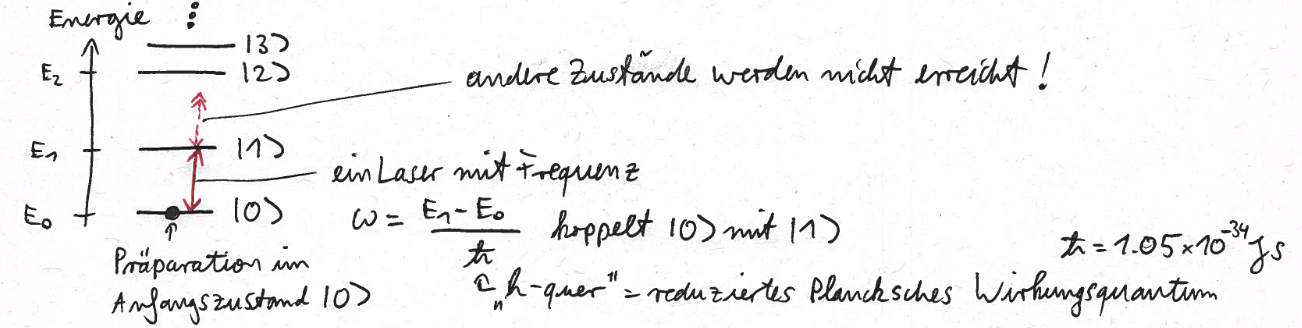
\includegraphics[width=.8\textwidth]{images/zustände.png}
\end{figure}
Mögliche Zustände des Qubits werden durch normierte Vektoren im von \ket{0} und \ket{1} aufgespannten 2-dimensionalen komplexen Vektorraum beschrieben:
\cf{
    \cket{\psi} = a_0\cket{0}+a_1\cket{1} = \matr{a_0\\a_1}\qquad a_0,a_1\in\mathbb{C}\text{ mit }|a_0|^2+|a_1|^2=1\text{ (Normierung)}
}

\subsubsection*{Messung}
Um Informationen über den Zustand des Qubits zu gewinnen, können wir eine Messung durchführen. Diese geschieht stets bezüglich einer bestimmten Orthonormalbasis, welche durch den Aufbau der Messapparatur bestimmt wird. Im Quantencomputing betrachtet man normalerweise nur Messungen bzgl. der Standardbasis (\ket{0} oder \ket{1}). Das Ergebnis der Messung ist \b{zufällig}, und zwar:
\begin{align*}
    p_0 &= |\skal{0}{\psi}|^2 = |(1,0)\matr{a_0\\a_1}|^2 = |a_0+0\cdot a_1|^2 = |a_0|^2\qquad\text{ Wahrscheinlichkeit für Ergebnis "0"}\\
    p_1 &= |\skal{1}{\psi}|^2 = |(0,1)\matr{a_0\\a_1}|^2 = |0\cdot a_0+a_1|^2 = |a_1|^2\qquad\text{ Wahrscheinlichkeit für Ergebnis "1"}
\end{align*}

\b{Nach der Messung} befindet sich das Qubit dann in dem Zustand, der dem gemessenen Ergebnis entspricht, d.h. \f{\cket{\psi}=\cket{0}} oder \f{\cket{\psi}=\cket{1}} ("Zustandsreduktion"). Eine Messung in der \ac{qm} hat also folgende Eigenschaften:
\begin{itemize}
    \item Ergebnis ist zufällig (wobei die Wahrscheinlichkeit für die verschiedenen möglichen Ergebnisse vom Zustand \ket{\psi} abhängen)
    \item Der Zustand \ket{\psi} wird durch die Messung verändert ("Kollaps des Quantenzustands")
\end{itemize} 
\vspace{1em}
\b{Frage:} Wer oder was entscheidet, ob das Ergebnis "0" oder "1" ausgewählt wird?\\
\f{\quad\rightarrow\quad} Antwort unbekannt! ("Messproblem" in der \ac{qm})\\
\vspace{1cm}

Für eine Messung bzgl. einer beliebigen Orthonormalbasis (\ket{v_1},\ket{v_2}) mit \f{|\skal{v_i}{v_j}|=\delta_{ij}} gilt entsprechend:
\cf{
    p_{v_i} = |\skal{v_i}{\psi}|^2\quad\text{Wahrscheinlichkeit für Messergebnis "}v_i\text{" } (i = 1,2)
}
Die Messung geht einer mit der entsprechenden Reduktion des Zustands:
\cf{
    \underbrace{\cket{\psi}}_{\text{Zustand vor der Messung}}\rightarrow\underbrace{\cket{v_i}}_{\text{Zustand nach der Messung mit Ergebnis "}v_i\text{" (i=1\text{ oder }2)}}
}

\subsubsection*{Dichteoperator und Invarianz bzgl. globaler Phase}
Betrachten wir einen beliebigen Zustand \ket{\psi} eines Qubits sowie \f{\cket{\psi^\prime}=e^{i\varphi}\cket{\psi}} mit \f{\varphi\in\mathbb{R}}, dann gilt:
\cf{
    p_{v_i}^\prime = |\skal{v_i}{\psi^\prime}|^2 = |e^{i\varphi}\skal{v_i}{\psi}|^2 = \underbrace{|e^{i\varphi}|^2}_{=1}\underbrace{|\skal{v_i}{\psi}|^2}_{=p_{v_i}} = p_{v_i}
}
Dies zeigt, dass \ket{\psi} und \ket{\psi^\prime} dieselbe Wahrscheinlichkeit für Messung in beliebiger Basis liefern!\\
Wir definieren nun den zu \ket{\psi} gehörigen Operator ("Dichteoperator" oder "Dichtematrix"):
\cf{
    \varrho = \cket{\psi}\cbra{\psi} = \matr{a_0\\a_1}\matr{a_0^* & a_1^*} = \matr{|a_0|^2 & a_0a_1^*\\a_1a_0^* & |a_1|^2} \qquad \text{(Darstellung bzgl. Standardbasis)}
}
\b{Achtung:} Der Dichteoperator ist nicht zu verwechseln mit dem Skalarprodukt:
\cf{\skal{\psi}{\psi} = \matr{a_0^*&a_1^*}\matr{a_0\\a_1} = |a_0|^2 + |a_1|^2 \in \mathbb{C}}
Der Dichteoperator liefert eine eindeutige Beschreibung der Wahrscheinlichkeiten für Messungen in beliebiger Basis:
\cf{
    p_{v_i} = |\skal{v_i}{\psi}|^2 = \skal{v_i}{\psi} \skal{v_i}{\psi}^* = \langle v_i\underbrace{\cket{\psi}\ \cbra{\psi}}_{=\varrho}v_i\rangle = \left\langle v_i|\varrho|v_i\right\rangle
}
Insbesondere sind die zu \ket{\psi} bzw. \ket{\psi^\prime} gehörigen Dichteoperatoren identisch:
\begin{gather*}
    \cket{\psi} = \matr{a_0\\a_1}\quad,\quad\cbra{\psi}=\matr{a_0^*&a_1^*}\quad,\quad\cket{\psi^\prime}=e^{i\varphi}\matr{a_0\\a_1}=\matr{e^{i\varphi} a_0\\e^{i\varphi} a_1}\quad,\quad\cbra{\psi^\prime}=\matr{e^{-i\varphi}a_0^* & e^{-i\varphi}a_1^*}\\
    \Rightarrow \varrho^\prime = \cket{\psi^\prime}\cbra{\psi^\prime} = e^{i\varphi}\cket{\psi}\cbra{\psi}e^{-i\varphi} = \cket{\psi}\cbra{\psi} = \varrho
\end{gather*}

\subsubsection*{Zustandstomographie eines Qubits}
Können wir den Zustand eines Qubits durch Messung bestimmen? Eine einzelne Messung reicht hierfür nicht aus; wir brauchen Mittelwerte über viele Messungen, um Wahrscheinlichkeiten abschätzen zu können. Da jedoch jede Messung den Zustand eines Qubits verändert, muss nach jeder Messung das Qubit erneut im ursprünglichen Zustand präpariert werden. Um den Dichteoperator \f{\varrho=\cket{\psi}\cbra{\psi}} eines Qubits vollständig zu bestimmen, benötigen wir Messungen in 3\footnote{Warum 3? - Um die 3 Komponenten des Blochvektors zu messen.} verschiedenen Orthonormalbasen.

\subsubsection*{Bloch-Vektor}
Wir definieren folgende 3 Operatoren (so genannte "Pauli-Operatoren"):
\cf{
    X = \matr{0&1\\1&0}\quad,\quad Y=\matr{0&-i\\i&0}\quad,\quad Z=\matr{1&0\\0&-1}
}

Die Pauli-Operatoren haben folgende Eigenschaften:
\begin{itemize}
    \item Selbstadjungiert: \f{X=X^\dagger, Y=Y^\dagger, Z=Z^\dagger}
    \item Spur=null: Tr(\f{X}) \f{=} Tr(\f{Y}) \f{=} Tr(\f{Z}) \f{=0}
    \item $\begin{aligned}[t]
        & XY=iZ   && , \quad YZ=iX   && , \quad ZX=iY \\
        & YX=-iZ  && , \quad ZY=-iX  && , \quad XZ=-Y
    \end{aligned}$
    \item \f{X^2=Y^2=Z^2=\mathbb{I}}
\end{itemize}
Mit Hilfe der Pauli-Operatoren kann die Dichtematrix eines Qubits anschaulich als dreidimensionaler, reeller Vektor dargestellt werden.
\definition{Blochvektor}{
    Für normierte Zustände \f{\varrho} mit Tr(\f{\varrho}) \f{=1} ist der Blochvektor definiert als:
    \begin{equation}
        \overrightarrow{s} = \matr{s_X\\s_Y\\s_Z}\quad\text{ wobei }\qquad\begin{matrix}
            s_X = \text{Tr}(\varrho X)\\
            s_Y = \text{Tr}(\varrho Y)\\
            s_Z = \text{Tr}(\varrho Z)
        \end{matrix}
    \end{equation}
    Umgekehrt gilt:
    \begin{equation}
        \varrho = \frac{1}{2}(\mathbb{I}+s_XX+s_YY+s_ZZ)
    \end{equation}
}
\b{Beweis:}
\begin{align*}
    \text{Tr}(\varrho X) &= \frac{1}{2}(\tr{\mathbb{I}X}+ s_X\tr{XX}+s_Y\tr{YX}+s_Z\tr{ZX})\\
    &= \frac{1}{2}(\tr{X} + s_X\tr{\mathbb{I}} - is_Y\tr{Z} + is_Z\tr{Y}) \\
    &= \frac{1}{2}2s_X = s_X\qquad\checkmark\quad\text{(ebenso für \f{\tr{\varrho Y}} und \f{\tr{\varrho Z}})}\\
    \tr{\varrho} &= \frac{1}{2}\tr{\mathbb{I}} = 1\qquad\checkmark
\end{align*}
Damit ist gezeigt: (Eq. 2) erfüllt die Gleichungen (Eq. 1) und die Bedingung \f{\tr{\varrho}=1}.\\
Die Eindeutigkeit von (Eq. 2) folgt aus der linearen Unabhängigkeit der Operatoren \f{\mathbb{I}, X, Y} u. \f{Z}. \f{\square}
\vspace{0.5cm}

\begin{minipage}{.48\textwidth}
\b{Blochkugel}
\begin{center}
    
\includegraphics[width=.95\textwidth]{images/blochsphere.png}
\end{center}
\end{minipage}
\begin{minipage}{.5\textwidth}
\begin{tabular}{c|c|c}
    \toprule
    \textbf{Zustandsvektor} & \textbf{Dichtematrix} & \textbf{Blochvektor} \\
    \midrule
    $|0\rangle = \begin{pmatrix} 1 \\ 0 \end{pmatrix}$ & 
    $\begin{pmatrix} 1 & 0 \\ 0 & 0 \end{pmatrix}$ & 
    $\begin{pmatrix} 0 \\ 0 \\ 1 \end{pmatrix}$ \\[2ex]

    $|1\rangle = \begin{pmatrix} 0 \\ 1 \end{pmatrix}$ &
    $\begin{pmatrix} 0 & 0 \\ 0 & 1 \end{pmatrix}$ &
    $\begin{pmatrix} 0 \\ 0 \\ -1 \end{pmatrix}$ \\[2ex]

    $|+\rangle = \frac{1}{\sqrt{2}} \begin{pmatrix} 1 \\ 1 \end{pmatrix}$ &
    $\frac{1}{2} \begin{pmatrix} 1 & 1 \\ 1 & 1 \end{pmatrix}$ &
    $\begin{pmatrix} 1 \\ 0 \\ 0 \end{pmatrix}$ \\[2ex]

    $|-\rangle = \frac{1}{\sqrt{2}} \begin{pmatrix} 1 \\ -1 \end{pmatrix}$ &
    $\frac{1}{2} \begin{pmatrix} 1 & -1 \\ -1 & 1 \end{pmatrix}$ &
    $\begin{pmatrix} -1 \\ 0 \\ 0 \end{pmatrix}$ \\[2ex]

    $|+i\rangle = \frac{1}{\sqrt{2}} \begin{pmatrix} 1 \\ i \end{pmatrix}$ &
    $\frac{1}{2} \begin{pmatrix} 1 & -i \\ i & 1 \end{pmatrix}$ &
    $\begin{pmatrix} 0 \\ 1 \\ 0 \end{pmatrix}$ \\[2ex]

    $|-i\rangle = \frac{1}{\sqrt{2}} \begin{pmatrix} 1 \\ -i \end{pmatrix}$ &
    $\frac{1}{2} \begin{pmatrix} 1 & i \\ -i & 1 \end{pmatrix}$ &
    $\begin{pmatrix} 0 \\ -1 \\ 0 \end{pmatrix}$ \\
    \bottomrule
\end{tabular}
\end{minipage}

\vspace{0.5cm}
Die Zeichnung zeigt 6 verschiedene Zustände auf der Blochkugel (siehe Tabelle). Orthogonale Zustände (wie \ket{0} und \ket{1}) befinden sich an entgegengesetzten Enden. Im Allgemeinen kann ein Zustand durch 2 Winkel \f{\vartheta} und \f{\varphi} beschrieben werden:
\cf{
    \cket{\psi} = \matr{\cos(\frac{\vartheta}{2})\\\sin(\frac{\vartheta}{2})e^{i\varphi}},\quad\varrho = \cket{\psi}\cbra{\psi} = \matr{\cos^2(\frac{\vartheta}{2})&\cos(\frac{\vartheta}{2})\sin(\frac{\vartheta}{2})e^{-i\varphi}\\\cos(\frac{\vartheta}{2})\sin(\frac{\vartheta}{2})e^{i\varphi}&\sin^2(\frac{\vartheta}{2})},\quad\overrightarrow{s}=\matr{\sin(\vartheta)\cos(\varphi)\\\sin(\vartheta)\sin(\varphi)\\\cos(\vartheta)}
}

\subsubsection*{Reine und gemischte Zustände}
Bislang haben wir den zu einem normierten Zustandsvektor \ket{\psi} (mit \f{\left\Vert\cket{\psi}\right\Vert = \sqrt{\skal{\psi}{\psi}} = 1}) gehörigen Dichteoperator \f{\varrho} wie folgt definiert: \f{\quad\varrho=\cket{\psi}\cbra{\psi}}\\
Ein solcher Zustand heißt \it{reiner Zustand}. Man kann zeigen, dass der Blochvektor \f{\overrightarrow{s}} eines reinen Zustands Betrag 1 hat, d.h. auf der Oberfläche der Blochkugel liegt:
\cf{
    |\overrightarrow{s}| = \sqrt{s_X^2 + s_Y^2+ s_Z^2} = 1
}
Es gibt aber auch Zustände im Inneren der Blochkugel (also \f{|\overrightarrow{s}| < 1}). Diese heißen \it{gemischte Zustände}. Ein Beispiel hierfür ist der sogenannte "maximale gemischte Zustand", der genau im Inneren der Blochkugel liegt (also \f{\overrightarrow{s}=\matr{0&0&0}^\top }). Gemäß (Eq. 2) lautet die dazugehörige Dichtematrix:
\cf{\varrho=\frac{1}{2}\mathbb{I}=\matr{\frac{1}{2}&0\\0&\frac{1}{2}}}
Dieser hat die besondere Eigenschaft, dass bei jeder beliebigen Messung (d.h. bzgl. einer beliebigen Basis \f{(\cket{v_1}, \cket{v_2})}) beide möglichen Ergebnisse mit Wahrscheinlichkeit \f{\frac{1}{2}} auftreten:
\cf{
    p_{v_i} = \left\langle v_i|\varrho|v_i\right\rangle = \langle v_i|\frac{1}{2}\mathbb{I}|v_i\rangle = \frac{1}{2}\langle v_i|\underbrace{\mathbb{I}\ |v_i}_{=\cket{v_i}}\rangle = \frac{1}{2}\underbrace{\skal{v_i}{v_i}}_{=1} = \frac{1}{2}\qquad(i=1,2)
}
Im allgemeinen muss eine Dichtematrix \f{\varrho} folgende Eigenschaften erfüllen:
\begin{enumerate}
    \item \b{Positivität:} (genauer: "positive Semidefinitheit")
    \cf{\left\langle \psi|\varrho|\psi\right\rangle \geq 0\quad\text{ für alle Zustandsvektoren }\cket{\psi}}
    (weil \f{\left\langle \psi|\varrho|\psi\right\rangle} die Wahrscheinlichkeit ist, bei einer Messung bzgl. einer Basis, die den Vektor \f{\cket{\psi}} enthält, das Messergebnis "\f{\cket{\psi}}" zu erhalten)
    \item \b{Normierung:} (weil sich die Wahrscheinlichkeiten zu 1 addieren müssen)
    \cf{
        \varrho = \matr{\varrho_{00}&\varrho_{01}\\\varrho_{10}&\varrho{11}}\ ,\quad\tr{\varrho} = \varrho_{00}+\varrho_{11} = 1
    }
    Hierbei ist \f{\varrho_{00} =\langle 0|\varrho|0\rangle} die Wahrscheinlichkeit für das Messergebnis "0", und \f{\varrho_{11}=\langle 1|\varrho|1\rangle} die Wahrscheinlichkeit für Messergebnis "1".
    \item \b{Selbstadjungiertheit:}\\
    Da für einen beliebigen linearen Operator \f{A} gilt: \f{A = A^\dagger \Leftrightarrow \langle\psi|A|\psi\rangle\in\mathbb{R}} für alle \ket{\psi}, folgt aus (1): \f{
        \varrho = \varrho^\dagger
    }.
\end{enumerate}
Wie schon erwähnt, liefert der Dichteoperator eine vollständige und eindeutige Beschreibung des Zustands eines Quantensystems, da durch ihn die Wahrscheinlichkeiten für alle möglichen Messungen definiert sind.\\
Beim Quantencomputing haben wir es jedoch meistens nur mit reinen Zuständen zu tun, also mit Zuständen der Form \f{\varrho = \cket{\psi}\cbra{\psi}}. In diesem Fall ist es praktischer, direkt mit dem Vektor \ket{\psi} zu arbeiten (da ein Vektor weniger Koeffizienten als eine Matrix hat):
\cf{
    \cket{\psi} = \matr{a_0\\a_1}\quad,\quad\varrho=\matr{|a_0|^2&a_0a_1^*\\a_1^*a_0&|a_1|^2}
}
\b{Beachte:} Wendet man einen Operator \f{A} auf einen Vektor \ket{\psi} an (\f{\cket{\psi}^\prime=A\cket{\psi}}), so lautet die entsprechende Operation für den Dichteoperator wie folgt:
\cf{
    \varrho^\prime = \cket{\psi^\prime}\cbra{\psi^\prime} = A\cket{\psi}\cbra{\psi}A^\dagger = A\varrho A^\dagger
}

\vspace{1cm}
\subsubsection*{Interpretation von \f{\varrho} als Zustandsgemisch}
Wir betrachten einen beliebigen Dichteoperator \f{\varrho} eines \f{d}-dimensionalen Quantensystems (für ein Qubit gilt \f{d=2}). Wegen \f{\varrho = \varrho^\dagger} ist \f{\varrho} unitär diagonalisierbar, d.h. es gibt eine Orthonormalbasis von Eigenvektoren von \f{\varrho}. Die Matrix \f{\varrho} lässt sich dann wie folgt schreiben:
\cf{
    \varrho = \sum_{i=1}^{d}p_i\cket{\psi_i}\cbra{\psi_i}\quad\text{("Spektralzerlegung")}
}
Hierbei ist \f{p_i} der \f{i}-te Eigenwert und \f{\cket{\psi_i}\cbra{\psi_i}} ein Projektor auf Eigenzustand \ket{\psi_i}.\\

\b{Interpretation:} \f{\varrho} ist ein statistisches Gemisch, bei dem Zustand \ket{\psi_i} mit Wahrscheinlichkeit \f{p_i} auftritt. Da \f{\varrho} positiv ist, gilt nämlich \f{p_i = \langle\psi_i|\varrho|\psi_i\rangle\geq 0}, und aus \f{\tr{\varrho} = 1} folgt \f{\sum_{i=1}^{d}p_i = 1}. Ein Beispiel hierfür ist der maximal gemischte Zustand:
\begin{gather*}
    \varrho_* = \frac{1}{2}\mathbb{I} = \matr{\frac{1}{2}&0\\0&\frac{1}{2}} = \frac{1}{2}\cket{0}\cbra{0}+\frac{1}{2}\cket{1}\cbra{1}\\
    \Rightarrow\quad\text{Zustand \ket{0} mit Wahrscheinlichkeit \f{\frac{1}{2}}, ebenso Zustand \ket{1}}
\end{gather*}
Der maximal gemischte Zustand ist von folgendem Zustand zu unterscheiden:
\begin{gather*}
    \varrho_+ = \cket{+}\cbra{+} = \frac{1}{2}\matr{1\\1}\matr{1&1} = \frac{1}{2}\matr{1&1\\1&1} = \matr{1/2&1/2\\1/2&1/2}\\
    \langle0|\varrho_+|0\rangle = 1/2\quad,\quad\langle1|\varrho_+|1\rangle=1/2
\end{gather*}
Eine Messung bzgl. der Basis (\ket{0}, \ket{1}) liefert zwar dasselbe Ergebnis wie für \f{\varrho_*} (nämlich Wahrscheinlichkeit \f{1/2}), aber für eine Messung bzgl. einer anderen Basis, z.B. (\ket{+}, \ket{-}) gilt:
\begin{align*}
    &\langle+|\varrho_*|+\rangle = \frac{1}{2}\langle+|\mathbb{I}|+\rangle = \frac{1}{2}\underbrace{\skal{+}{+}}_{=1} = 1/2\\
    &\text{jedoch:}\quad\langle+|\varrho_+|+\rangle = \underbrace{\skal{+}{+}}_{=1}\underbrace{\skal{+}{+}}_{=1} = 1
\end{align*}
Es gibt folgendes einfaches Kriterium, um reine von gemischten Zuständen zu unterscheiden: Sei \f{\varrho} eine Dichtematrix, dann gilt:
\begin{gather*}
    \varrho \text{ ist ein reiner Zustand }\Leftrightarrow \tr{\varrho^2} = 1\\
    \varrho \text{ ist ein gemischter Zustand }\Leftrightarrow \tr{\varrho^2} < 1\\
\end{gather*}
\subsubsection*{Messung einer Observablen}
Die Sprechweise "Messung bzgl. einer Basis \dots" ist etwas umständlich und wenig gebräuchlich. Meistens spricht man stattdessen von "Messung einer Observablen" wie folgt:
\begin{itemize}
    \item[-] Eine Observable ist ein selbstadjungierter Operator \f{A=A^\dagger}
    \begin{flalign*}
        \Rightarrow A = \sum_ia_i\cket{\psi_i}\cbra{\psi_i}\quad\text{(Spektralzerlegung) (\f{a_i} sind reelle EW von \f{A}; \f{\cket{\psi_i}} die EV)}&&
    \end{flalign*}
    \item[-] Die Messung von \f{A} entspricht der Messung bzgl. der Eigenzustände \f{\left\{\cket{\psi_i}\right\}} von \f{A}. Ergebnis der Messung ist der entsprechende Eigenwert \f{a_i\in\mathbb{R}}.
    \item[-] Der \it{Erwartungswert von \f{A} im Zustand \f{\varrho}} ergibt sich daraus wie folgt:
    \begin{flalign*}
        (1)\ \text{"Einfügen der Eins":}\quad\mathbb{I} = \sum_j\cket{j}\cbra{j} = \matr{1&0\\0&1} &&
    \end{flalign*}
    \vspace{-0.7cm}
    \begin{flalign*}
        \langle A\rangle &= \sum_ip_ia_i = \sum_i\langle\psi_i|\varrho|\psi_i\rangle a_i \stackrel{(1)}{=} \sum_{i,j}\langle\psi_i|\varrho|j\rangle\langle j|\psi_i\rangle a_i = \sum_j\langle j|\Sigma_ia_i|\psi_i\rangle\langle\psi_i|\varrho|j\rangle && \\
        &= \langle j|A\varrho|j\rangle = \tr{A\varrho} && 
    \end{flalign*}
\end{itemize}


\subsubsection*{Mehrere Qubits}
Das Zusammensetzen mehrerer einzelner Systeme zu einem Gesamtsystem geschieht in der \ac{qm} mit dem \it{Tensorprodukt}.\\
Betrachten wir 2 Qubits, jedes mit Basiszuständen \ket{0} und \ket{1}, so lautet die Basis für das Gesamtsystem:
\begin{align*}
    \cket{0} &\otimes \cket{0}\quad\text{(beide Qubits in Zustand \ket{0})}\\
    \cket{0} &\otimes \cket{1}\quad\text{(erstes Qubit in \ket{0}, zweites in \ket{1})}\\
    \cket{1} &\otimes \cket{0}\quad\text{usw.}\\
    \cket{1} &\otimes \cket{1}
\end{align*}
Zustandsvektoren von 2 Qubits sind also im allgemeinen Linearkombinationen dieser 4 Basiszustände:
\begin{gather*}
    \cket{\psi}=a_{00}\cket{0}\otimes\cket{0}+a_{01}\cket{0}\otimes\cket{1}+a_{10}\cket{1}\otimes\cket{0}+a_{11}\cket{1}\otimes\cket{1}\\
    \text{mit }a_{00},a_{01},a_{10},a_{11}\in\mathbb{C}\text{ und }|a_{00}|^2+|a_{01}|^2+|a_{10}|^2+|a_{11}|^2=1
\end{gather*}
Das Symbol für das Tensorprodukt "\f{\otimes}" wird häufig weggelassen, d.h. man schreibt "\f{\cket{0}\cket{0}}" oder, noch einfacher, "\f{\cket{00}}" anstelle von "\f{\cket{0}\otimes\cket{0}}".\\
Für \f{n} Qubits erhält man entsprechend \f{2^n} Basiszustände:
\begin{gather*}
    \left\{\cket{00\dots00},\cket{00\dots01},\cket{00\dots10},\dots,\cket{11\dots11}\right\}\quad\text{bzw.}\\
    \left\{\cket{i_1i_2\dots i_n}\ |\ i_1=0,1;\ i_2=0,1;\ \dots;\ i_n=0,1\right\}
\end{gather*}
Zustandsvektor für \f{n} Qubits:
\begin{align*}
    \cket{\psi} &= a_{00\dots00}\cket{00\dots00} + a_{00\dots01}\cket{00\dots01} + a_{00\dots10}\cket{00\dots10}+\dots+a_{11\dots11}\cket{11\dots11}\\
    &= \sum_{i_1=0,1}\sum_{i_2=0,1}\dots\sum_{i_n=0,1}a_{i_1i_2\dotsi_n}\cket{i_1i_2\dots i_n}\\
    &= \sum_{i=0}^{2^n-1}a_i\cket{i}
\end{align*}
In der letzten Zeile werden die Basiszustände mittels \f{i=0,1,\dots,2^n-1} durchgezählt, wobei:
\begin{align*}
    i &= 2^{n-1}i_1+2^{n-2}i_2+\dots+2^{1}i_{n-1}+2^0i_n\\
    &= \sum_{k=1}^{n}2^{n-k}i_k\qquad\text{(Binärdarstellung)}
\end{align*}
\subsubsection*{Messung an mehreren Qubits}
\begin{itemize}
    \item Misst man den Zustand aller Qubits (Basis \f{\left\{\cket{i}, i=0,1,\dots,2^{n}-1\right\}}), so gilt wie gehabt:
    \begin{gather*}
        p_i = |\skal{i}{\psi}|^2\qquad\text{Wahrscheinlichkeit für Ergebnis "}i\text{",}
    \end{gather*}
    wobei \ket{\psi} der Zustandsvektor der \f{n} Qubits vor der Messung, und \ket{i} der Zustandsvektor der Qubits nach der Messung ist (bzw. \f{p_i=\cbra{i}\varrho\cket{i}}, falls sich die Qubits in einem gemischten Zustand befinden). Beipiel (für 2 Qubits):
    \begin{gather*}
        \cket{\psi} = a_{00}\cket{00}+a_{01}\cket{01}+a_{10}\cket{10}+a_{11}\cket{11}\\
        \Rightarrow p_{00} = |a_{00}|^2\qquad\text{(Wahrscheinlichkeit, beide Qubits in "0" zu messen)}
    \end{gather*}
    \item Misst man den Zustand nur teilweise (z.B. nur für 1 Qubit), erhält man dasselbe Ergebnis wie als ob man alle Qubits misst und über die möglichen Ergebnisse der anderen Qubits summiert.\\
    Obiges Beispiel: Wahrscheinlichkeit, das erste Qubit in "0" zu messen:
    \begin{gather*}
        p_{0.} = |a_{00}|^2 + |a_{01}|^2\qquad\text{(zweites Qubit in "0" oder "1")}
    \end{gather*}
    \item Die Summierung über alle möglichen Zustände eines Teilsystems nennt man auch die "partielle Spur". Deren allgemeine Definition ist wie folgt: Wir betrachten ein Gesamtsystem, das aus zwei Teilsystemen \f{A} und \f{B} zusammengesetzt ist (z.B. \f{A=} Qubit 1, \f{B=} Qubit 2).\\
    Das Gesamtsystem befinde sich im Zustand \(\varrho_{AB}\). Daraus ergibt sich der \it{Zustand des Teilsystems A} durch die partielle Spur \it{über Teilsystem B}:
    \begin{gather*}
        \varrho_A = \text{Tr}_B(\varrho_{AB})
    \end{gather*}
    wobei \f{\varrho_A} durch seine Matrixelemente wie folgt definiert ist:
    \begin{gather*}
        \cbra{i}\varrho_A\cket{i} = \sum_k\cbra{i,k}\varrho_{AB}\cket{j,k}\qquad\text{(Summe über Basis \f{\left\{\cket{k}\right\}} von System \f{B})}
    \end{gather*}
    \item \b{Zustandsreduktion bei Messung an einem Teilsystem}\\
    Erinnerung: Messung an Gesamtsystem mit Basis \f{\left\{\cket{i}\right\}\quad\Rightarrow\quad\cket{\psi}\xrightarrow[\text{Ergebnis }i]{\text{Messung}}\cket{i}}\\
    Dies kann man verstehen als Anwendung des Projektors \f{P_i=\cket{i}\cbra{i}}, gefolgt von Normierung:
    \begin{gather*}
        \cket{\psi}\rightarrow P_i\cket{\psi} = \cket{i}\skal{i}{\psi} \xrightarrow{\text{Normierung}}\cket{i}\\
        \shortintertext{(wobei das Betragsquadrat der Norm der Wahrscheinlichkeit für Ergebnis \f{i} enspricht)}
        \Vert P_i\cket{\psi}\Vert^2 = \Vert\ \cket{i}\skal{i}{\psi}\Vert^2 = \underbrace{|\skal{i}{\psi}|}_{P_i}{^2}\ \underbrace{\Vert\cket{1}\Vert}_{=1}{^2}=P_i
    \end{gather*}
    Bei Messung an einem Teilsystem hat Projektor die Form: 
    \begin{gather*}
        P_i = \underbrace{\cket{i}\cbra{i}}_{\text{gemessenes System, Ergebnis \f{i}}}\otimes\underbrace{\mathbb{I}}_{\text{nicht gemessenes System, da} \sum_iP_i = \mathbb{I}}
    \end{gather*}
    Zustandsreduktion: 
    \begin{gather*}
        \cket{\psi}\rightarrow\frac{P_i\cket{\psi}}{\Vert\ P_i\cket{\psi}\Vert}
    \end{gather*}
    \b{Beispiel:}
    \begin{gather*}
        \cket{\psi} = a_{00}\cket{00}+ a_{01}\cket{01}+ a_{10}\cket{10}+a_{11}\cket{11}\\
        \shortintertext{Nach Messung des ersten Qubits in $\cket{0}$ erhalten wir: 
        $P_0 = \cket{0}\cbra{0}\otimes\mathbb{I}$}
        P_0\cket{\psi} = a_{00}\cket{00}+a_{01}\cket{01} 
        \qquad(\Vert P_0\cket{\psi}\Vert^2 = |a_{00}|^2+|a_{01}|^2 = \text{ WSK für Ergebnis }\cket{0})\\
        \shortintertext{Der Zustand nach der Messung lautet:}
        \frac{a_{00}\cket{00}+a_{01}\cket{01}}{\sqrt{|a_{00}|^2+|a_{01}|^2}}
        = \cket{0}\otimes\frac{1}{\sqrt{|a_{00}|^2+|a_{01}|^2}}
        (a_{00}\cket{0}+a_{01}\cket{1})
    \end{gather*}
    \item \b{Verschränkung}\\
    Sei \f{\varrho_{AB}=\cket{\psi_{AB}}\cbra{\psi_{AB}}} ein reiner Zustand. \f{\cket{\psi_{AB}}} heißt Produktvektor, wenn es Vektoren \f{\cket{\psi_A}} bzw. \f{\cket{\psi_B}} in Teilsystemen \f{A} bzw. \f{B} gibt, so dass \f{\cket{\psi_{AB}} = \cket{\psi_A}\otimes\cket{\psi_B}}.\\
    Ansonsten heißt \f{\cket{\psi_{AB}}} verschränkt. In den Übungen wurde gezeigt:
    \begin{gather*}
        \cket{\psi_{AB}}\text{ Produktvektor }\Rightarrow\varrho_A\text{ reiner Zustand (ebenso \f{\varrho_B})}
    \end{gather*}
    Dies gilt auch umgekehrt (siehe z.B. Nielsen/Chuang), also:
    \begin{gather*}
        \cket{\psi_{AB}}\text{ Produktvektor} \Leftrightarrow \varrho_A\text{ reiner Zustand (ebenso \f{\varrho_B})}
    \end{gather*}
    Mit anderen Worten: Falls \ket{\psi_{AB}} verschränkt ist (und nur dann), befinden sich die Teilsysteme jeweils in einem gemischten Zustand, obwohl der Zustand des Gesamtsystems rein ist!
    \item \b{Dekohärenz durch Verschränkung mit der Umgebung}\\
    Wenn ein System mit seiner Umgebung wechselwirkt, kann es sich (und wird es sich typischerweise) mit dieser verschränken. Der Zustand des Systems ist dann nicht mehr rein, sondern gemischt.\\
    Für das Quantencomputing brauchen wir jedoch reine Zustände. Daher müssen die Qubits gut von ihrer Umgebung isoliert werden. Den Verlust der Reinheit bezeichnet man auch als "Dekohärenz". Sie stellt für die praktische Umsetzung des Quantencomputings ein entscheidendes Problem dar (mögliche Lösung: Quantenfehlerkorrektur).
\end{itemize}


















\section{Funktionsweise eines gatterbasierten Quantencomputers}
Es gibt 4 allgemeine Konzepte für Quantencomputer (QC):
\begin{itemize}
    \item Gatterbasiere Quantencomputer (z.B. IBM)
    \item Adiabatischer Quantencomputer (z.B. DWave)
    \item Quantensimulatoren
    \item Einweg-Quantencomputer
\end{itemize}
Der gatterbasierte QC ist ein besonders flexibles Konzept, und man kann mit ihm im Prinzip alle Rechnungen durchführen, die auch mit den anderen Konzepten möglich sind.

\subsection{Klassischer Computer (Schaltkreismodell)}
Eine Rechnung auf einem klassischen Computer lässt sich auf einige elementare logische Operationen zurückführen, welche den Zustand (0 oder 1) von einem oder zwei Bits manipulieren:

\cig{.7}{gates1}
\cig{.7}{gates2}

Jede Funktion \f{\left\{0,1\right\}^n\rightarrow\left\{0,1\right\}^m} (\f{n, m}: Anzahl der Bits für input bzw. output) kann hiermit berechnet werden. Beweis: siehe Vorlesungsfolien (Seite 30f).


\subsection{Universalität von NAND and COPY}
NAND and COPY reichen aus, um alle anderen Gatter zu erzeugen, insbesondere NOT, AND und XOR (die im obigen Beweis der Konstruktion einer beliebigen Booleschen Funktion verwendet wurden).

\cig{.7}{gates3}

\subsection{Komplexität von Berechnungen}
Wie lange braucht ein Algorithmus, um die Lösung eines Problems zu finden? Die benötigte Zeit \f{T} ist synonym zur Anzahl der logischen Gatter.
\begin{itemize}
    \item \b{Klasse P}: Zeit wächst polynomial mit der Länge \f{n} des Inputs (\f{n} = Anzahl der Bits, um den Input darzustellen). Beispiele: Addition zweier Zahlen (\f{T\propto n}), Multiplikation (\f{T\propto n^2}).\\
    Solche Probleme gelten als "einfach" bzw. "schnell lösbar", im Gegensatz zu Problemen, bei denen \f{T} exponentiell mit \f{n} wächst und welche daher für großes \f{n} praktsich unlösbar sind.
    \item \b{Klasse NP}: Probleme, deren Lösung möglicherweise schwer zu finden ist, bei denen sich aber schnell (d.h. in polynomieller Zeit) prüfen lässt, ob eine gegebene vorgeschlagene Lösung richtig ist. Beispiel: Faktorisierung ganzer Zahlen (für große Zahlen \f{N} schwer zu finden, aber für gegebene Faktoren \f{p} und \f{q} kann man leicht prüfen, ob \f{N=pq}).
    \item \b{Klasse NP-vollständig}: Teilmenge von NP mit der folgenden besonderen Eigenschaft: falls ein NP-vollständiges Problem in Zeit \f{T} gelöst werden kann, kann jedes andere NP-Problem in Zeit \f{T'=\textrm{Polynom}(T)} gelöst werden.\\Beispiel: Travelling-Salesman-Problem (kürzeste Route zwischen \f{N} Städten).
\end{itemize}

Eines der wichtigsten ungelösten Probleme der Informatik ist die Frage ob P=NP? Wahrscheinlich ist dies nicht der Fall (sonst wäre z.B. das Faktorisierungsproblem schnell lösbar), aber bis jetzt gibt es dafür keinen Beweis!\\
Mit einem Quantencomputer kann das Faktorisierungsproblem in Polynomialzeit gelöst werden. Man vermutet jedoch (aber bisher ohne Beweis), dass NP-vollständige Probleme auch von Quantencomputern \b{nicht} in Polynomialzeit gelöst werden können.

\subsection{Gatterbasierte Quantencomputer}
Allgemeine Funktionsweise: Die Rechnung erfolgt in 3 Schritten.
\begin{enumerate}
    \item Präparation des Anfangszustands (alle Qubits im Zustand \ket{0}):
    \cf{\cket{\psi_0} = \cket{0}\otimes\cket{0}\otimes\dots\otimes\cket{0}=\cket{0}^{\otimes n}=\cket{00\dots 0}}
    \item Anwendung einer unitären Operation \f{U} erzeugt den Endzustand: \f{\cket{\psi} = U\cket{\psi_0}}\\
    \f{U} muss unitär sein, damit \ket{\psi} normiert ist!
    \cf{\skal{\psi}{\psi} = \langle\psi_0|\underbrace{U^\dagger U}_\mathbb{I}|\psi_0\rangle = \skal{\psi_0}{\psi_0} = 1}
    \item Messung des Endzustands in Standardbasis (\ket{0}, \ket{1}) für jedes Qubit:\\
    \f{\rightarrow} Ergebnis \f{i=i_1i_2...i_n\ (i=0,1,2,...,2^n\ ;\ i_1,...,i_n=0,1)} mit WSK \f{p_i=|\skal{i}{\psi}|^2} 
\end{enumerate}
\cig{.4}{qc}

Ähnlich wie beim klassischen Computer kann man auch beim Quantencomputer die Rechenoperation \f{U} in eine kleine Menge elementarer logischer Operationen (1- und 2-Qubit-Gatter) zerlegt werden.\\
Bei der Messung stellt sich das grundsätzliche Problem, dass das Messergebnis i.a. zufällig ist. Verschiedene Quantenalgorithmen gehen hiermit auf unterschiedliche Weise um:
\begin{itemize}
    \item Manchmal kann der Algorithmus so konstruiert werden, dass das gewünschte Ergebnis mit 100\% Wahrscheinlichkeit auftritt.
    \item In anderen Fällen wird der Alorithmus so lange wiederholt, bis das gewünschte Ergebnis gemessen wird. Voraussetzungen, damit dies funktioniert:
    \begin{itemize}
        \item für eine gegebene Lösung \f{i_1i_2...i_n} kann man leicht prüfen, ob diese richtig ist (z.B. bei Problemen der Klasse NP).
        \item die WSK, eine richtige Lösung zu messen, muss groß genug sein.
    \end{itemize}
    \item In wiederum anderen Fällen besteht das Ergebnis des Quantenalgorithmus aus einem Mittelwert über viele Messungen.
\end{itemize}


\subsection{1-Qubit-Gatter}
Wir besprechen nun die Bausteine, aus denen wir "Quantenschaltkreise" (d.h. unitäre Operationen \f{U}) konstruieren können. Als erstes zählen wir einige Gatter auf, die nur auf einzelne Qubits wirken:
\begin{itemize}
    \item \b{X-Gatter:} Entspricht dem klassischen NOT-Gatter. Auf der Blochkugel bewirkt X eine Rotation von 180° um die X-Achse. 
    \cf{X = \matr{0&1\\1&0} = \cket{0}\cbra{1}+\cket{1}\cbra{0}}
    \item \b{Y-Gatter:} Rotation 180° um die Y-Achse
    \cf{Y = \matr{0&-i\\i&0}}
    \item \b{Z-Gatter:} Rotation 180° um die Z-Achse
    \cf{Y = \matr{1&0\\0&-1}}
    \item \b{Hadamard-Gatter:} Rotation 180° um den Vektor \f{(1\ 0\ 1)^T}. 
    \cf{
        H = \frac{1}{\sqrt{2}}\matr{1&1\\1&-1} = \cket{+}\cbra{0}+\cket{-}\cbra{1}}
    \cf{
        H\cket{0} = \frac{1}{\sqrt{2}}\left(\cket{0}+\cket{1}\right) = \cket{+}\quad,\quad H\cket{1} = \frac{1}{\sqrt{2}}\left(\cket{0}-\cket{1}\right) = \cket{-}
    }
    \cf{H^2=\mathbb{I}\quad,\quad HXH=Z\quad,\quad HZH=X}
    Viele Quantenalgorithmen beginnen damit, auf jedes Qubit ein Hadamard-Gatter anzuwenden. Dies erzeugt eine gleichmäßige Superposition aller \f{2^n} Basiszustände.
    \begin{flalign*}
        H^{\otimes n}\cket{0}^{\otimes n} & = (H\cket{0})^{\otimes n}  = \left(\frac{1}{\sqrt{2}}(\cket{0}+\cket{1})\right)^{\otimes n} \\
        & = \frac{1}{\sqrt{2^n}}(\cket{00...00}+\cket{00...01}+...+\cket{11...11}) = \frac{1}{\sqrt{2^n}}\sum_{j=0}^{2^n-1}\cket{j}
    \end{flalign*}
    \item \b{Phasengatter:} Parametrisiertes Gatter (d.h. abhängig von Parameter \f{\varphi}). Rotation von Winkel \f{\varphi} um Z-Achse (\f{\varphi = \pi} entspricht 180°)
    \cf{
        R_\varphi = \matr{1&0\\0&e^{i\varphi}}\quad,\quad R_\pi = Z
    }
    \item \b{S/T-Gatter:} Rotationsgatter mit jeweils \f{\varphi = \frac{\pi}{2}} und \f{\varphi = \frac{\pi}{4}}.
    \cf{
        S = R_{\frac{\pi}{2}} = \matr{1&0\\0&i}\quad,\quad S^2=Z
    }
    \cf{
        T = R_{\frac{\pi}{4}} = \matr{1&0\\0&\frac{1+i}{\sqrt{2}}}\quad,\quad T^2=S
    }
    \item \b{Pauli-Rotationsgatter:}
    \begin{flalign*}
        R_X(\varphi) = e^{-i\frac{\varphi}{2}X}\quad\rightarrow\quad\textrm{Rotation Winkel }\varphi\textrm{ um X-Achse}\\
        R_Y(\varphi) = e^{-i\frac{\varphi}{2}Y}\quad\rightarrow\quad\textrm{Rotation Winkel }\varphi\textrm{ um Y-Achse}\\
        R_Z(\varphi) = e^{-i\frac{\varphi}{2}Z}\quad\rightarrow\quad\textrm{Rotation Winkel }\varphi\textrm{ um Z-Achse}
    \end{flalign*}
\end{itemize}
In den Übungen zeigen wir \f{R_Z(\varphi) = e^{-i\frac{\varphi}{2}}R_\varphi}, d.h. die Gatter \f{R_Z(\varphi)} und \f{R_Y} sind bis auf eine globale Phase zueinander äquivalent! Da eine solche globale Phase letztlich irrelevant ist, sind die beiden Gatter physikalisch miteinander identisch und entsprechen derselben Rotation auf der Blochkugel. Außerdem zeigen wir in den Übungen:
\begin{flalign*}
    XYX = -Y\quad\quad &,\quad\quad XZX = -Z\\
    XR_Y(\varphi)X = R_Y(-\varphi)\quad\quad &,\quad\quad XR_Z(\varphi)X = R_Z(-\varphi)
\end{flalign*}

\subsubsection{Allgemeines 1-Qubit-Gatter}
Jedes 1-Qubit-Gatter kann (bis auf eine globale Phase) wie folgt mit Hilfe von 3 Parametern (\f{\vartheta, \varphi, \lambda}) geschrieben werden:
\cf{
    U_3(\vartheta, \varphi, \lambda) = \matr{
        \cos(\frac{\vartheta}{2})&-e^{i\lambda}\sin(\frac{\vartheta}{2})\\
        e^{i\varphi}\sin(\frac{\vartheta}{2})&e^{i\lambda + i \varphi}\cos(\frac{\vartheta}{2})
    }
}
In den Übungen zeigen wir:
\cf{
    U_3(\vartheta, \varphi, \lambda) = \underbrace{e^{i\frac{\varphi + \lambda}{2}}}_{\textrm{globale Phase}}\overbrace{R_Z(\varphi)R_Y(\vartheta)R_Z(\lambda)}^{\textrm{Rotation um z- und y-Achse}}
}
Daraus ergibt sich folgendes Korollar, welches im nächsten Kapitel nützlich sein wird: Jedes 1-Qubit-Gatter \f{U} kann wie folgt dargestellt werden (Beweis: siehe Übungen):
\cf{
    U = e^{i\alpha}AXBXC
}
Hierbei sei \f{\alpha\in\mathbb{R}} ein Phasenfaktor und \f{A, B} und \f{C} jeweils 1-Qubit-Gatter mit \f{ABC=\mathbb{I}}.












\subsection{2-Qubit-Gatter: CNOT}
Das CNOT-Gatter ("controlled-NOT") funkioniert wie folgt:
\begin{itemize}
    \item Falls das control-qubit im Zustand \ket{0} ist, passiert nichts.
    \item Falls das control-qubit im Zustand \ket{1} ist, wird die Operation NOT (bzw. X) auf das target-qubit angewandt.
\end{itemize}

\begin{figure}[h!]
\centering
\begin{subfigure}{.5\textwidth}
  \centering
  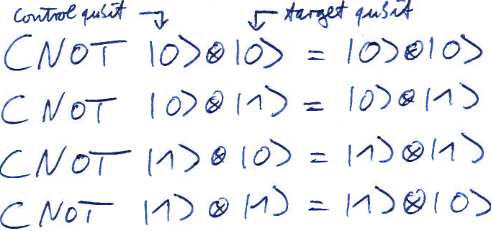
\includegraphics[width=.7\linewidth]{cnot}
\end{subfigure}%
\begin{subfigure}{.5\textwidth}
  \centering
  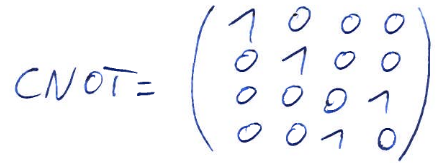
\includegraphics[width=.7\linewidth]{cnot2}
\end{subfigure}
\end{figure}

Das CNOT-Gatter bildet zusammen mit den 1-Qubit-Gattern eine \b{universelle Menge} von Quantengattern, d.h. jede unitäre Operation auf \f{n} Qubits kann durch CNOT und 1-Qubit-Gatter erzeugt werden. (Hier weggelassen: Beweis)\\
Im allgemeinen kann jede unitäre Operation \f{U} auf 2 Qubits mit Hilfe von 3 CNOT-Gattern und 8 1-Qubit-Gattern erzeugt werden:

\cig{.6}{universell}

Ein Beispiel, für das 3 CNOT-Gatter benötigt werden, ist das SWAP-Gatter: \cf{\textrm{SWAP}\ \cket{\psi}\otimes\cket{\chi} = \cket{\chi}\otimes\cket{\psi}}

\begin{figure}[h!]
\centering
\begin{subfigure}{.5\textwidth}
  \centering
  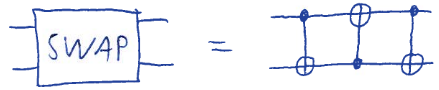
\includegraphics[width=.7\linewidth]{swap}
\end{subfigure}%
\begin{subfigure}{.5\textwidth}
  \centering
  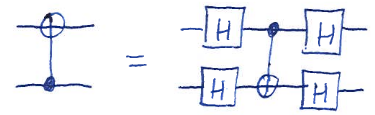
\includegraphics[width=.6\linewidth]{swap2}
\end{subfigure}
\end{figure}

Beim 2. CNOT ist hier die Rolle von control und target vertauscht. Manchmal lässt die QC-Hardware das CNOT-Gatter jedoch nur in einer Richtung zu. Die Umkehrung kann dann wie rechts in der obigen Abbildung erreicht werden.\\
SWAP-Gatter spielen im Quantencomputing eine wichtige Rolle, welche mit der "Konnektivität" der Qubits zu tun hat. In der Quantencomputer-Hardware sind nämlich CNOT-Gatter meistens nur zwischen bestimmten Paaren von Qubits implementiert. Beispiel: 5-Qubit ibmq-vigo

\cig{.9}{swap3}

Da jedes SWAP-Gatter 3 CNOTs benötigt, sind dies insgesamt 13 CNOTs! Dies ist wichtig, da die CNOT-Gatter im allgemeinen die größte Fehlerquelle darstellen (2025: ca. 0.2\% für 2-Qubit-Gatter).\\
Zum Schluss geben wir noch ein Beispiel für ein 3-Qubit-Gatter an, und wie dieses mit Hilfe von CNOT- und 1-Qubit-Gattern realisiert werden kann: Für ein beliebiges 1-Qubit-Gatter \f{U} definieren wir das zweifach kontrollierte \f{U}-Gatter \f{C_2U} wie folgt:

\cig{.6}{cnot3}

Für das Gatter werden insgesamt 8 CNOT-Gatter benötigt (da CV bzw. CV\f{^\dagger} jeweils 2 CNOT-Gatter enthält).\\

Ein allgemeines Rezept, wie man eine beliebige unitäre Operation auf \f{n} Qubits mit CNOT- und 1-Qubit-Gattern erzeugen kann, wird z.B. im Buch von Nielsen/Chuang angegeben. Allerdings benötigt man im allgemeinen hierfür eine exponentiell große Anzahl von Gattern. Für Quantencomputing sind hingegen nur solche Schaltkreise von praktischem Nutzen, bei denen die Anzahl der Gatter polynomial mit \f{n} skaliert. Wie man eine gegebene Operation optimal (d.h. mit möglichst wenigen 1- und 2-Qubit-Gattern) darstellt, ist ein schwieriges, noch ungelöstes Problem.

\subsection{Simulierbarkeit durch klassische Computer}
Im allgemeinen kann man einen Quantenschaltkreis mit genügend vielen Qubits (\f{n>50...60}) nicht auf einem klassischen Computer simulieren. Dies scheitert daran, dass der Quantenzustand (Dimension \f{2^n}) nicht mit dem verfügbaren Speicherplatz dargestellt werden kann. Es gibt folgende Ausnahmen:
\begin{itemize}
    \item \b{Nur 1-Qubit Gatter:} Der Quantenzustand bleibt dann immer ein Produktzustand\\
    \f{\cket{\psi_1}\otimes\cket{\psi_2}\otimes...\otimes\cket{\psi_n}}, welcher mit \f{2n} statt \f{2^n} Parametern dargestellt werden kann.
    \item \b{Clifford-Gatter:} Hierzu zählen \f{X,Y,Z,H,S} und CNOT. Quantenschaltkreise, die nur mit diesen Gattern erzeugt werden, können ebenfalls effizient auf klassischen Computern simuliert werden. Clifford-Gatter bilden Pauli-Matrizen auf Pauli-Matrizen ab (ein Gegenbeispiel ist T).
\end{itemize}

\subsubsection{n-Qubit-Pauli-Operatoren}
n-Qubit-Pauli-Operatoren sind Produkte der 1-Qubit-Pauli-Operatoren X,Y,Z und \(\mathbb{I}\). Ein Beispiel: \f{P = X\otimes\mathbb{I}\otimes Z = X_1Z_3} ist ein 3-Qubit-Pauli-Operator (X auf Qubit 1 und Z auf Qubit 3).\\
Ein Gatter ist ein Clifford-Gatter, wenn für alle Pauli-Operatoren P gilt: \f{CPC^\dagger=P'}, wobei \f{P'} ebenfalls ein Pauli-Operator ist. Die Simulation eines nur aus Clifford-Gattern bestehenden Schaltkreises funktioniert deshalb wie folgt:
\begin{itemize}
  \item Anfangszustand \ket{00...0} ist Eigenzustand der \f{n} Pauli-Operatoren \f{Z_1, Z_2,...,Z_n} jeweils zum\\Eigenwert +1, also:
  \begin{flalign*}
    Z_1\cket{00...0} = \cket{00...0}\quad, ...,\quad Z_n\cket{00...0} = \cket{00...0}     
  \end{flalign*}
  \item Der Zustand \f{\cket{\psi} = C\cket{00...0}} ist dann Eigenzustand von \f{CZ_1C^\dagger=P_1}, \f{CZ_2C^\dagger=P_2} usw., da:
  \cf{
    CZ_1C^\dagger\cket{\psi} = CZ_1C^\dagger C\cket{00...0} = CZ_1\cket{00...0} = C\cket{00...0}=\cket{\psi}
  }
  \item Ebenso gilt nach Anwendung weiterer Clifford-Gatter \f{C'}: Ist \ket{\psi} Eigenzustand von \f{P_1,...,P_n}, so ist \f{\cket{\psi'}=C'\cket{\psi}} Eigenzustand von \f{P_1', ..., P_n'}, wobei \f{P_i'=C'P_iC'^\dagger}
  \item Der Zustand des \f{n}-Qubit-Registers kann also im Computer durch \f{n} Pauli-Operatoren dargestellt werden, wobei jeder Pauli-Operator nur \f{2n} Bits benötigt (4 Möglichkeiten, also 2 Bit pro Qubit: \f{X,Y,Z} oder \f{\mathbb{I}}).
  \item Die Simulation des Messprozesses (in der Standardbasis) ist in diesem Formalismus ebenfalls möglich (siehe Nielsen/Chuang).
\end{itemize}

\subsection{Klassische Berechnungen auf dem Quantencomputer}
Umgekehrt kann jedoch jede klassische Rechnung auf einem Quantencomputer mit einer der Anzahl klassischer Bits vergleichbaren Anzahl Qubits durchgeführt werden.\\

Wir betrachten z.B. die Berechnung einer Funktion \f{f(x)\in\left\{0,1\right\}}, wobei der Input \f{x} aus \f{n} Bits besteht. Für diese Funktion \f{f} existiert dann ein klassischer Schaltkreis, der aus elementaren Gattern wie NOT, AND, XOR usw. besteht. Der zu \f{f} gehörige Quantenschaltkreis \f{U_f} ist wie folgt definiert:
\cf{U_f\cket{x}\otimes\cket{0}=\cket{x}\otimes\cket{f(x)}}
Um \f{U_f} aus dem klassischen Schaltkreis zu konstruieren, sehen wir uns zunächst einige elementare Gatter an:
\cig{.65}{u_f}

Man beachte, dass das AND-Gatter die Einführung eines 3. Hilfsqubits (auch "Ancilla"-Qubit genannt) erfordert, um eine reversible Operation zu erhalten (Quantengatter sind stets unitär, d.h. umkehrbar, da \f{UU^\dagger=\mathbb{I}\Rightarrow U^{-1}=U^\dagger}). Beispielsweise wäre die Operation \f{A\cket{x,y}=\cket{x,x\wedge y}} nicht reversibel, da \f{A\cket{0,0}=A\cket{0,1}=\cket{0,0}}.\\
Setzt man \f{\cket{y}=\cket{0}} beim XOR-Gatter, kann man das klassische COPY-Gatter realisieren: 
\cf{\textrm{CNOT}\cket{x,0}=\cket{x,x}}
Das "No-Cloning-Theorem" besagt, dass nur die Zustände \ket{0} und \ket{1} kopiert werden können, nicht beliebige Superpositionen \ket{\psi}. Ein Gatter \f{U} mit \f{U\cket{\psi,0}=\cket{\psi,\psi}} für ein beliebiges \f{\cket{\psi}} kann es nicht geben!\\
Mit den obigen elementaren Gattern können wir nun folgenden Schaltkreis konstruieren, wobei evtl. eine gewisse Anzahl \f{m} von Ancilla-Qubits benötigt wird:
\cig{.6}{o_f}
Das Output-Qubit befindet sich im Zustand \ket{f(x)}. Der Zustand \ket{g(x)} ist beliebig und im folgenden ohne Belang. Wir kopieren das Output-Qubit und stellen durch den inversen Schaltkreis \f{O_f^{-1}} den Anfangszustand wieder her (Symbol "/" ist ein aus mehreren Qubits bestehendes Register):
\cig{.6}{o_f2}

Die \f{m} Ancilla-Qubits bleiben im Zustand \ket{0} und werden im folgenden außer Acht gelassen. Für die restlichen Qubits gilt nun:
\cf{
  \cket{x}\otimes\cket{0}\quad\longrightarrow\quad\cket{x}\otimes\cket{f(x)}
}
Also genau wie der oben definierte Schaltkreis \f{U_f}!\\[1em]

Kann man in einem Quantenalgorithmus auch direkt \f{O_f} statt \f{U_f} verwenden und auf das Wiederherstellen des Anfangszustands mittels \f{O_f^{-1}} verzichten? Nein, denn 
dies kann aufgrund des unbekannten Zustands \ket{g(x)} zu falschen Ergebnissen führen, falls man mit Superpositionszuständen rechnet. Falls z.B. \f{\cket{g(x_1)}=\cket{g(x_2)}=:g}, so gilt:
\cf{
  O_f\cket{0}\otimes(\cket{x_1}+\cket{x_2}) = \cket{g}\otimes(\cket{f(x_1)}+\cket{f(x_2)})\quad\Rightarrow\quad\textrm{Output-Qubit in reinem Zustand}
}
Ansonsten gilt:
\cf{
  O_f\cket{0}\otimes(\cket{x_1}+\cket{x_2}) = \cket{g(x_1)}\otimes\cket{f(x_1)}+\cket{g(x_2)}\otimes\cket{f(x_2)}\quad\Rightarrow\quad\textrm{Output-Qubit in gemischtem Zustand}
}

\subsection{Deutsch-Algorithmus}
Wir kommen nun zu unserem ersten Quantenalgorithmus: der Deutsch-Algorithmus ist der einfachste Quantenalgorithmus, der eine bestimmte Aufgabe effizienter als ein klassischer Algorithmus lösen kann, und daher gut für illustrative Zwecke geeignet, auch wenn die durch ihm gelöste Aufgabe keinen bekannten praktischen Zweck erfüllt.\\[0.5em]
\b{Aufgabe:} Für eine gegebene Funktion \f{f:\left\{0,1\right\}\rightarrow\left\{0,1\right\}}, welche in Form einer blackbox vorliegt (z.B. eines in seiner internen Funktion unbekannten elektronischen Schaltkreises), finde heraus, ob \f{f(0)=f(1)} (konstant) oder \f{f(0)\neq f(1)} (alternierend).\\
Klassisch muss der Schaltkreis für \f{f} zweimal durchlaufen werden, um sowohl \f{f(0)} als auch \f{f(1)} zu berechnen. Quantenmechanisch muss der zu \f{f} gehörige Quantenschaltkreis nur \b{einmal} durchlaufen werden. Dieser Schaltkreis realisiert folgende unitäre Operation auf einem Register von 2 Qubits:
\cf{
  U_f\cket{i}\otimes\cket{j}=\cket{i}\otimes\cket{j\oplus f(i)}
}
Hierbei ist \f{\oplus} die binäre Addition (d.h. modulo 2). Das Register braucht 2 Qubits, damit \f{U_f} unitär ist. Die Operation \f{\cket{i}\rightarrow\cket{f(i)}} mit 1 Qubit wäre nicht unitär, falls \f{f} konstant ist. Z.B. \f{f(0)=f(1)=0} würde folgender Matrix entsprechen:
\cf{
  f = \matr{1&1\\0&0}\quad\textrm{wobei}\quad ff^\dagger = \matr{1&1\\0&0}\matr{1&0\\1&0}=\matr{2&0\\0&0}\neq\mathbb{I}
}

\cig{1}{deutsch}
Die Messung (4) liefert also mit 100\% WSK das Ergebnis "0", wenn \f{f} konstant ist, bzw. "1" falls \f{f} alternierend ist (Herleitung weggelassen). \\
Dieses Beispiel illustriert die Idee des "Quantenparallelismus" (d.h. eine Funktion \f{f(x)} kann gleichzeitig für verschiedene Argumente \f{x} ausgewertet werden). Wir sehen aber auch, dass der Algorithmus auf eine spezielle Art konstruiert werden muss, damit zum Schluss ein eindeutiges Messergebnis die Lösung des Problems liefert.










\section{Quantenalgorithmen}
In diesem Kapitel stellen wir einige Algorithmen vor, die für Anwendungen interessant sein können, d.h. bei denen der Quantencomputer einen Vorteil gegenüber dem klassischen Computer verspricht.

\subsection{Grover-Suchalgorithmus}
Dieser Algorithmus beschleunigt die Suche nach einem bestimmten Element in einer unstrukturierten Menge von Elementen. Beispiele:
\begin{itemize}
    \item Suche nach einer bestimmten Telefonnummer in einem nach Namen sortierten Telefonbuch
    \item Suche nach der kürzesten Verbindung zwischen \f{K} Städten
\end{itemize}

\subsubsection{Allgemeine Formulierung}
Für eine gegebene Funktion \f{f: \left\{0,1\right\}^n\rightarrow\left\{0,1\right\}}, suche \f{x} (\f{2^n} mögliche Inputs für \f{x}), so dass \f{f(x)=1}.\\[0.5em]
Anwendung (z.B.) auf das Traveling-Salesman-Problem: Jeder Input bezeichnet eine mögliche Route (Anzahl \f{(K-1)!\leq N = 2^n}), dann ist \f{f(x)} definiert durch:
\cf{
    f(x) = \begin{cases}
        0\quad\textrm{falls Länge der Route} > L\\
        1\quad\textrm{falls Länge der Route} \leq L
    \end{cases}
}
Die kürzeste Route kann dann gefunden werden, indem man verschiedene Werte von \f{L} probiert.

\subsubsection{Orakel}
Ähnlich wie beim Deutsch-Algorithmus wird zur Funktion \f{f} ein Quantenschaltkreis \f{O} ("Orakel") konstruiert:
\cf{
    \cket{x}\cket{q}\ \xmapsto{O}\ \cket{x}\cket{q\oplus f(x)}\quad\quad\begin{aligned}
        &x = 0,1,2,...,2^n-1\ \quad(n\textrm{ Qubits})\\
        &q = 0,1\ \quad(1\textrm{ Qubit})
    \end{aligned}
}
Hierzu nehmen wir an, dass zur Berechnung von \f{f} ein effizienter klassischer Schaltkreis existiert (z.B. ist bei Traveling-Salesman die Berechnung der Länge einer gegebenen Route leicht möglich). Dieser kann dann auf einem entsprechenden Quantenschaltkreis von ungefähr gleicher Komplexität abgebildet werden. 
Das Orakel-Qubit \ket{q} wird im Zustand \f{\cket{q}=\frac{1}{\sqrt{2}}(\cket{0}-\cket{1})} initialisiert. Dann gilt:
\cf{
    \cket{x}(\frac{\cket{0}-\cket{1}}{\sqrt{2}})\ \xmapsto{O}\ \begin{cases}
        \cket{x}(\frac{\cket{0}-\cket{1}}{\sqrt{2}})\quad\textrm{falls }f(x)=0 \\
        \cket{x}(\frac{\cket{1}-\cket{0}}{\sqrt{2}})\quad\textrm{falls }f(x)=1
    \end{cases}
}
\cf{
    \Rightarrow\ \cket{x}(\frac{\cket{0}-\cket{1}}{\sqrt{2}})\ \xmapsto{O}\ (-1)^{f(x)}\cket{x}(\frac{\cket{0}-\cket{1}}{\sqrt{2}})
}
Das Orakel-Qubit bleibt im selben Zustand und wird im folgenden außer Acht gelassen. Somit gilt:
\cf{
    \cket{x}\ \xmapsto{O}\ (-1)^{f(x)}\cket{x}
}

\subsubsection{Grover-Iteration}
Wir nehmen nun an, dass die Anzahl \f{M} der gesuchten Lösung (Elemente \f{x}, für die gilt \f{f(x)=1}) bekannt ist (falls nicht, gibt es einen anderen Quantenalgorithmus "Quantum Counting", der \f{M} berechnen kann). Der Suchalgorithmus funktioniert dann wie folgt:
\begin{enumerate}
    \item Anwendung von \f{H} auf jedes Qubit erzeugt gleichförmige Überlagerung aller Basiszustände:
    \cf{
        H^{\otimes n}\cket{0} = \cket{\psi_0} = \frac{1}{\sqrt{N}}\sum_{j=0}^{N-1}\cket{j}\qquad\quad(N=2^n)
    }
    \item Ca. \f{\sqrt{\frac{N}{M}}}-fache Anwendung der Grover-Unterroutine \f{G} (siehe unten)
    \item Messung aller Qubit ergibt Kandidaten \f{x} für gesuchte Lösung
\end{enumerate}
\cig{.7}{grover}

\subsubsection{Grover-Unterroutine}
Diese enthält das Orakel und ein \f{(n-1)}-fach kontrolliertes Phasengatter von folgender Art, welches mit \f{\O (n)} elementaren Gattern erzeugt werden kann:
\cf{
    \cket{x}\ \rightarrow\ \begin{cases}
        \cket{x}\quad\textrm{falls }x=0\ \textrm{(alle Qubits in }\cket{0})\\
        -\cket{x}\quad\textrm{ansonsten}
    \end{cases}
}
\cig{.6}{grover2}

\subsubsection{Geometrische Visualisierung}
Die Funktionsweise des Grover-Algorithmus können wir am einfachsten anhand von Rotationen in einem zweidimensionalen Unterraum verstehen. Zu diesem Zweck definieren wir folgende zwei Zustände:

\cf{
    \cket{\alpha}=\frac{1}{\sqrt{N-M}}\sum_{\substack{\left\{x : f(x)=0\right\} \\\mathclap{\overset{\uparrow}{\text{Summe über alle "falschen" } x}}}}\cket{x}\qquad,\qquad
    \cket{\beta}=\frac{1}{\sqrt{M}}\sum_{\substack{\left\{x : f(x)=1\right\} \\\mathclap{\overset{\uparrow}{\text{Summe über gesuchte } x\text{ (Anzahl M)}}}}}\cket{x}
}

Der Anfangszustand \f{\cket{\psi_0}=H^{\otimes n}\cket{0}} ist eine Linearkombination dieser beiden Zustände:
\cf{
    \cket{\psi_0}=\frac{1}{\sqrt{N}}\sum_{x=0}^{N-1}\cket{x}=\underbrace{\sqrt{\frac{N-M}{N}}}_{=a_0}\cket{\alpha} + \underbrace{\sqrt{\frac{M}{N}}}_{=b_0}\cket{\beta}
}
Wegen \f{O\cket{x}=(-1)^{f(x)}\cket{x}} gilt mit \f{a,b\in\mathbb{R}} beliebig:
\f{
    O(a\cket{\alpha}+b\cket{\beta}) = a\cket{\alpha}-b\cket{\beta}
}\\
\f{\Rightarrow\ \text{Orakel spiegelt an }\cket{\alpha}\text{-Achse}}
\begin{figure}[h!]
    \centering
    \begin{subfigure}{.49\textwidth}
        \centering
        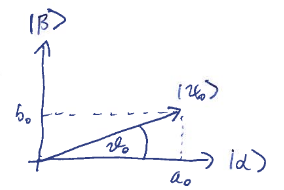
\includegraphics[width=.7\linewidth]{grover3}
    \end{subfigure}
    \begin{subfigure}{.49\textwidth}
        \centering
        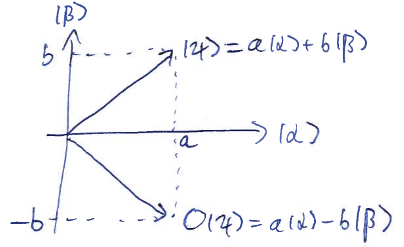
\includegraphics[width=.8\linewidth]{grover4}
    \end{subfigure}
\end{figure}

Den Diffusionsoperator \f{D} können wir wie folgt schreiben:
\cf{
    D = H^{\otimes n}\underbrace{(2\cket{0}\cbra{0}-\mathbb{I})}_{{\mathclap{\begin{aligned}
            \cket{0}\mapsto\cket{0} \quad&\text{da }(2\cket{0}\cbra{0}-\mathbb{I})\cket{0}=2\cket{0}-\cket{0}=\cket{0}\\
            \cket{x}\mapsto -\cket{x} \quad&\text{für }x>0\ (\Rightarrow \skal{0}{x}=0)
        \end{aligned} 
    }}}H^{\otimes n} = 2\cket{\psi_0}\cbra{\psi_0}-\mathbb{I}
}
Wegen \f{\cket{\psi_0}=a_0\cket{\alpha}+b_0\cket{\beta}} führt auch die Anwendung von \f{D} nicht aus dem von \ket{\alpha} und \ket{\beta} aufgespannten Unterraum hinaus!\\
Es gilt \f{D\cket{\psi_0}=2\cket{\psi_0}-\cket{\psi_0}=\cket{\psi_0}} und \f{D\cket{\chi_0}=-\cket{\chi_0}} für \f{\skal{\chi_0}{\psi_0}=0} (also \ket{\chi_0} senkrecht zu \ket{\psi_0}). Somit bewirkt \f{D} eine Spiegelung an \f{\psi_0}. Die Grover-Iteration \f{G^m=(DO)^m} spiegelt also abwechselnd and \ket{\alpha} bzw. \ket{\psi_0}!

\cig{.5}{grover5}

Jedes Anwendung von \f{G} führt zu einer Rotation um den Winkel \f{2\vartheta_0}. Daraus folgt:
\begin{gather*}
    \vartheta_m = \vartheta_0 + 2m\vartheta_0 = (1+2m)\vartheta_0\\
    \cket{\psi_m} = G^m\cket{\psi_0}=\sin(\vartheta_m)\cket{\beta}+\cos(\vartheta_m)\cket{\alpha}
\end{gather*}
Die WSK, nach \f{m} Iterationen eine gesuchte Lösung \f{f(x)=1} zu messen, ist gegeben durch:
\cf{
    p = \sum_{\{x:f(x)=1\}}|\skal{x}{\psi_m}|^2=\sum_{\{x:f(x)=1\}}|\sin(\vartheta_m)\frac{1}{\sqrt{m}}|^2=\sin^2(\vartheta_m)
}
Wir brauchen also \f{\vartheta_m=\frac{\pi}{2}}, um den Zustand in Richtung \ket{\beta} zu rotieren und \f{p\approx 1} zu erhalten. Die Anzahl der nötigen Iterationen lässt sich bestimmen durch:
\cf{
    (1+2m)\vartheta_0\approx\frac{\pi}{2}\quad\Rightarrow\quad m\approx\left(\frac{\pi}{2\vartheta_0}-1\right)\frac{1}{2}=\frac{\pi}{4\vartheta_0}-\frac{1}{2}\quad\text{with }\vartheta_0=\sin^{-1}(\sqrt{\frac{M}{N}})
}
Falls \f{N>>M}, dann ist \f{\sqrt{\frac{M}{N}}<<1\Rightarrow\vartheta_0\approx\sqrt{\frac{M}{N}}} (weil \f{\sin(x) \approx x} für \f{x<<1}), und somit:
\cf{
    m\approx\frac{\pi}{4}\sqrt{\frac{N}{M}}
}
Klassisch braucht man ungefähr \f{\frac{N}{M}} Versuche, um eine richtige Lösung zu finden, falls das Suchproblem "unstrukturiert" ist, d.h. es keine bessere Strategie als brute-force gibt. Somit bringt Grover eine Beschleunigung von \f{\frac{N}{M}\rightarrow\sqrt{\frac{N}{M}}} (nicht exponentiell schneller, aber evtl. doch relevant).


\subsection{Die Quantenfouriertransformation und ihre Anwendungen}
Wir besprechen zwei wichtige Algorithmen, die gegenüber den besten bekannten klassischen Algorithmen eine exponentielle Beschleunigung versprechen:
\begin{itemize}
    \item Faktorisierung ganzer Zahlen durch den Shor-Algorithmus
    \item Lösung linearer Gleichungssysteme durch den HHL-Algorithmus
\end{itemize}
Essentielle Bestandteile beider Algorithmen sind die Quantenfouriertransformation (QFT) und die Quantenphasenschätzung (QPE).

\definition{Klassische diskrete Fouriertransformation (DFT)}{
    Die DFT für \f{x_0, x_1, ..., x_{n-1}\in\mathbb{R}\ \xrightarrow{DFT}\ y_0, y_1, ..., y_{n-1}} ist definiert durch:
    \cf{
        y_k = \frac{1}{\sqrt{N}}\sum_{j=0}^{N-1}x_je^{2\pi ij\frac{k}{N}}
    }
}
Die Fouriertransformation hat zahlreiche Anwendungen z.B. in digitaler Signalverarbeitung wobei \f{x_i} ein zeitdiskretes Signal und \f{y_i} ein diskretes Frequenzspektrum wäre.\\

Falls das Eingangssignal periodisch ist (mit Periode \f{T}, und \f{N} ein Vielfaches von \f{T}), so kommen in der DFT nur die Frequenzen \f{\frac{N}{T}} und deren ganzzahlige Vielfache vor.
\cig{.8}{dft}

\subsubsection{Quantenfouriertransformation (QFT)}
Für die Standardbasisvektoren \f{\cket{j}=\cket{j_1j_2...j_n}} (\f{n} Qubits, \f{N=2^n}) (wobei \f{j=\sum_{k=1}^{n}2^{n-k}j_k} ,\\\f{j_k\in\{0,1\}}) definieren wir:
\cf{
    \text{QFT}\cket{j}=\frac{1}{\sqrt{N}}\sum_{k=0}^{N-1}e^{2\pi ij\frac{k}{N}}\cket{k}
}
Wendet man QFT auf eine Superposition \f{\sum_{j=0}^{N-1}x_j\cket{j}} an, erhält man also:
\cf{
    \text{QFT}\left(\sum_{j=0}^{N-1}x_j\cket{j}\right)=\sum_{k=0}^{N-1}\frac{1}{\sqrt{N}}\underbrace{\sum_{j=0}^{N-1}x_je^{2\pi ij\frac{k}{N}}}_{=y_k}\cket{k}=\sum_{k=0}^{N-1}y_k\cket{k}
}
\b{Bemerkung:} Die klassische DFT wird manchmal auch mit einem Minuszeichnen im Exponenten definiert (was dann der inversen Transformation entspricht). Dieses erhält man, indem man die Koeffizienten \f{x_j} und \f{y_j} komplex konjugiert:
\cf{
    y_k^*=\frac{1}{\sqrt{N}}\sum_{j=0}^{N-1}x_j^*e^{-2\pi ij\frac{k}{N}}
}
Der der QFT entsprechende Quantenschaltkreis ist wie folgt gegeben (Herleitung weggelassen) (Achtung: Reihenfolge der Qubits umgedreht):
\cig{.8}{qft}
Auf jedes Qubit \f{l\ (=1,2,...,n)} wenden wir also folgende Operationen an: Ein Hadamard-Gatter, dann eine Reihe von kontrollierten diskreten Phasengattern \f{R_2, R_3, ..., R_{n+1-l}} jeweils mit Qubit l+1, l+2, ..., n als Kontroll-Qubit. Die diskreten Phasengatter sind definiert durch:
\cf{
    R_k = \matr{1&0\\0&e^{2\pi \frac{i}{2k}}}
}
Am Schluss muss noch die Reihenfolge der Qubits umgedreht werden, um die QFT zu erhalten (Überprüfung S.75 weggelassen).\\[1em]
Die Zahl der Gatter in QFT ist \f{n(n+1)/2}. Klassisch brauchen wir \f{\approx 2^n} (exponentiell mehr) Gatter zur Berechnung der Fast-Fourier-Transform (FFT). Wir können jedoch nicht ohne weiteres QFT benutzen, um beliebige Anwendungen, welche klassische FT benötigen, zu beschleunigen.\\
Dies liegt daran, dass die Präparation des Anfangszustands (\f{\sum_{j=0}^{N-1}x_j\cket{j}\ ,\ N=2^n}) und die Messung der Amplituden \f{y_0,...,y_{N-1}} im Endzustand jeweils exponentiell viele Operationen erfordern. Trotzdem kann die QFT in einigen Fällen (bei denen der Anfangszustand leicht präpariert werden kann und zum Schluss nur wenige Amplituden gemessen werden müssen) nützlich sein, wie wir im folgenden sehen werden. 



\subsection{Quantenphasenschätzung (QPE)}
\b{Aufgabe:} Bestimme den Eigenwert \f{e^{2\pi i\varphi_u}} eines geg. imitären Operators \f{U} zum Eigenvektor \ket{u}. Hierzu brauchen wir:
\begin{itemize}
    \item Effiziente Schaltkreise ("Orakel"), um den Zustand \ket{u} zu präparieren und um kontrollierte \f{U^{2^j}}-Operationen durchzuführen.
    \item Ein zusätzliches Register von \f{t} Qubits, wobei \f{n} die Genauigkeit des Ergebnisses in Bits ist:
    \cf{
        t = n + \log(2+\frac{1}{2\epsilon})\qquad(\text{Erfolgs-WSK: }\geq 1-\epsilon)
    }
\end{itemize}
Der erste Schritt des QPE-Protokolls funktioniert wie folgt:
\cig{.8}{qpe}
Die kontrollierten \f{U^{2^j}}-Operationen (\f{j=0,...,t-1}) lassen den Zustand \ket{u} unverändert\\
(\f{U^{2^j}\cket{u}=e^{2\pi i2^j\varphi_u}\cket{u}}) und führen zu einem Phasenfaktor \f{e^{2\pi i2^j\varphi_u}}, falls das entsprechende Kontroll-Qubit im Zustand \ket{1} ist.\\
Falls die Phase \f{\varphi_u} mit \f{t} Qubits exakt ausgedrückt werden kann, d.h. falls \f{\varphi_u=\frac{j}{2^t}} mit ganzer Zahl \f{j=0,1,...,2^t}, dann stimmt der Zustand auf der rechten Seite mit QFT\ket{j} überein.\\
Wir führen also die inverse QFT (= QFT\f{^\dagger}) durch, und schreiben den QPE-Schaltkreis in kompakter Form wie folgt:
\cig{.8}{qpe2}
\vspace{1cm}
Falls \f{\varphi_u\neq\frac{j}{2t}}, dann liefert der obige Schaltkreis mit WSK \f{>1-\epsilon} eine \f{n}-Bit-Näherung von \f{\varphi_u}:
\cf{
    \cket{0}\cket{u}\xrightarrow{\text{QPE}}\cket{\tilde{\varphi_u}}\cket{u}
}
D.h. die Messung \f{\tilde{\varphi_u}} liefert (mit WSK \f{>1-\epsilon}) ein Messergebnis \f{j}, dessen erste \f{n} Bits mit den ersten \f{n} Bits von \f{2^t\varphi_u} übereinstimmen.\\
Falls der Zustand \ket{u} nicht genau präpariert werden kann und sich das 2. Register stattdessen anfangs in einer Überlagerung \f{\cket{\psi}=\sum_{u}c_u\cket{u}} verschiedener Eigenzustände befindet, so liefert QPE mit WSK \f{|c_u|^2} eine \f{n}-Bit Näherung von \f{\varphi_u}:
\cf{
    \cket{0}\cket{\psi}\xrightarrow{QPE}\sum_uc_u\cket{\tilde{\varphi_u}}\cket{u}
}


\subsection{Shor-Algorithmus}
\subsubsection{Faktorisierungsproblem}
\b{Aufgabe:} Gegeben sei eine natürliche Zahl \f{N}, welche keine Primzahl ist. Finde ganze Zahlen \f{p} und \f{q}, so dass \f{N=pq}.\\[0.5em]
Der beste bekannte klassische Algorithmus ("Zahlkörpersieb") benötigt \f{e^{1.7L^{1/3}(\ln L)^{2/3}}} (exponentielle) Operationen, um eine Zahl \f{N} mit \f{L} Bits (\f{L=\log_2 N}) zu faktorisieren. Shors Algorithmus benötigt lediglich \f{O(L^3)} Operationen. Dies hat schwere Konsequenzen für die Sicherheit des RSA public key Kryptografieverfahrens.

\subsubsection{Umformulierung: Ordnung modulo N}
Um mit dem Quantencomputer gelöst werden zu können, wird das Faktorisierungsproblem mit Hilfe von Zahlentheorie in ein äquivalentes Problem wie folgt umgeformt:
\begin{itemize}
    \item wähle zufällig eine ganze Zahl x zwischen 1 und \f{N-1}
    \item betrachte die Funktion: \f{f(r)=x^r\mod N}
\end{itemize}
\cig{.8}{shor}
Es fällt auf: \f{f(r)} ist periodisch mit Periode 4, wobei \f{f(4)=1}. Allgemein gilt: Falls \f{x} und \f{N} keinen gemeinsamen Teiler haben (ggT\f{(x,N)=1}), dann gibt es eine ganze Zahl \f{r<N}, so dass \f{f(r)=x^r\mod N = 1}.\\
Die kleinste Zahl mit dieser Eigenschaft heißt "Ordnung von \f{x} modulo \f{N}", und die Funktion \f{f} ist dann periodisch mit Periode \f{r}.\\

Nehmen wir nun an: \f{r} ist gerade und \f{x^{r/2}\mod N\neq N-1} (*). Dann gilt:
\cig{.7}{shor2}
Die beiden Zahlen \f{x^{r/2}-1} und \f{x^{r/2}+1} müssen also jeweils einen Faktor von \f{N} enthalten, und somit müssen ggT\f{(x^{r/2}-1,N)} und ggT\f{(x^{r/2}+1,N)} liefern jeweils einen Faktor von \f{N}.\\
Außerdem kann man zeigen, dass bei zufällig gewähltem \f{x} die Bedingung (*) mit WSK \f{\geq1/2} erfüllt ist, falls \f{N} keine gerade Zahl ist und \f{N\neq a^b} für ganze Zahlen \f{a} und \f{b}.\\

\b{Zusammenfassung:} \f{N} kann wie folgt faktorisiert werden:
\begin{enumerate}
    \item Falls \f{N} gerade ist oder \f{N=a^b}, gib 2 oder \f{a} als Faktor von \f{N} aus.
    \item Wähle zufällig \f{x} zwischen 1 und \f{N-1}. Falls ggT\f{(x,N)>1} gib diese Zahl als Faktor aus.
    \item Bestimme die Ordnung \f{r} von \f{x\mod N} mit dem unten beschriebenen Quantenalgorithmus.
    \item Falls \f{r} gerade ist und \f{x^{r/2}\mod N\neq N-1}, gib ggT\f{(x^{r/2}-1, N)} oder ggT\f{(x^{r/2}+1,N)} als Faktor von \f{N} aus. Falls nicht, gehe zurück zu (2).
\end{enumerate}
% Bis auf den 3. Schritt, können alle Schritte effizient auf einem klassischen Computer durchgeführt werden.\\
% \subsubsection{Funktionsweise}

\b{Beispiel:} \f{N=15\Rightarrow L=4} (da \f{2^4=16>15})\\
Die gesuchte Ordnung \f{r} kann Werte zwischen 1 und 15 annehmen. Aus unserem Messergebnis \f{j} erhalten wir \f{\varphi=j/2t} als Schätzung für \f{s/r}. Gesucht ist nun der Bruch \f{s/r} mit \f{r\leq15}, der am nächsten an unserer Schätzung \f{\varphi} liegt. Der kleinste Unterschied zwischen zwei Brüchen \f{s_1/r_1\neq s_2/r_2} beträgt:
\cig{.3}{shor3}
Die Genauigkeit der Schätzung \f{\varphi} muss also mindestens \f{\Delta/2=1/420} betragen, wozu \f{n\geq\log_2(420)=8.7}, also \f{n\geq 9\ (=2L+1)} Bits benötigt werden. Wählen wir also \f{t=9} Bits in Register 1 und erhalten als Messergebnis z.B. \f{j=147\ \Rightarrow\ \varphi = 147/2^9 = 147/512}. Entwickelt man \f{\varphi} als Kettenbruch:
\cig{.5}{shor4}
Lässt man Gleider des Kettenbruchs weg, erhält man Annäherungen an \f{\varphi} mit kleinerem Nenner:
\cf{
    \frac{1}{3}\approx0.333\quad,\quad \frac{1}{3+\frac{1}{2}}=\frac{2}{7}\approx0.285714\quad,\quad \frac{1}{3+\frac{1}{2+\frac{1}{14}}}=\frac{29}{101}\approx 0.287129
}
Die beste Näherung mit \f{r\leq 15} ist also \f{\frac{s}{r}=\frac{2}{7}=\frac{4}{14}\ \Rightarrow\ r=7} oder \f{r=14}.\\

Der Shor-Algorithus kann aus folgenden Gründen fehlschlagen:
\begin{itemize}
    \item \f{\varphi=\tilde{s}/r} ist eine schlechte Näherung an \f{s/r}. Dies geschieht mit Wahrscheinlichkeit \f{\leq\epsilon}, welche für genügend großes \f{t=2L+1+\log(2+\frac{1}{2\epsilon})} vernachlässigt werden kann.
    \item \f{s} und \f{r} haben einen gemeinsamen Faktor (z.B. \f{\frac{2}{7}=\frac{4}{14}}). Der Algorithmus muss dann wiederholt werden. Nielsen/Chuang zeigen, dass wenige Wiederholungen ausreichen, um mit hoher WSK die richtige Lösung zu erhalten.
\end{itemize}

\b{Benötigte Ressourcen:} Um eine Zahl \f{N} mit \f{L} Bits zu faktorisieren:
\begin{itemize}
    \item Zahl der Qubits: \f{L+t = 3L+3} (für \f{\epsilon<1/4})
    \item Zahl der Quantengatter: \f{O(L^3)}. Die meisten Gatter werden zur Berechnung der Funktion \f{x^k\mod N} benötigt.
\end{itemize}

Für kryptographisch relevante Schlüsselgrößen (\f{L}=1024,2048,...) wird Shors Algorithmus nicht ohne Quantenfehlerkorrektur funktionieren, welche wiederum eine große Anzahl zusätzlicher Qubits erfordert. Laut einer aktuellen Schätzung werden ca. 20 Millionen fehlerbehaftete Qubits (Fehlerrate \f{10^{-3}}) benötigt, um eine 2048-Bit Zahl in 8 Stunden zu faktorisieren. 


\subsection{HHL-Algorithmus}
\b{Aufgabe:} Lösung eines linearen Gleichungssystems, d.h. zu gegebener Matrix \f{A\in\mathbb{C}^{N\times N}} und Vektor \f{\vec{b}\in\mathbb{C}^N}, finde \f{\vec{x}\in\mathbb{C}^N}, so dass \f{A\vec{x}=\vec{b}}.
\begin{itemize}
    \item Dies entspricht der Invertierung der Matrix \f{A: \vec{x}=A^{-1}\vec{b}}
    \item Falls \f{A} selbstadjungiert ist (\f{A=A^\dagger}), erhalten wir mit Hilfe der Spektralzerlegung:
    \cf{
        A = \sum_{i=1}^{N}\lambda_i\cket{v_i}\cbra{v_i}\Rightarrow A^{-1}=\sum_{i=1}^{N}\lambda_i^{-1}\cket{v_i}\cket{v_i}
    }
\end{itemize}
\subsubsection{Laufzeit auf einem klassischen Computer}
Mit dem Verfahren der konjugierten Gradienten, erreichen klassiche Computer:
\cf{
    O(Ns\kappa\log(\frac{1}{\epsilon}))
}
Wobei \f{s} die "sparseness" von \f{A} (höchstens \f{s} Matrixeinträge ungleich Null pro Spalte oder Zeile) bezeichnet, \f{\kappa=\frac{G_{max}}{G_{min}}} die Kondition der Matrix \f{A} (\f{G_i} sind Singulärwerte von \f{A}), und \f{\epsilon} die Genauigkeit der Lösung.

\subsubsection{Quantenalgorithmus (HHL)}
\begin{itemize}
    \item Laufzeit: \f{O(\log(N)s^2\kappa^2/\epsilon)} (exponentielle Beschleunigung in \f{N})
    \item 1. Annahme: \f{A=A^\dagger} (ansonsten, löse \f{\matr{0&A\\A^\dagger&0}\matr{0\\\vec{x}}=\matr{\vec{b}\\0}})
    \item 2. Annahme: Es gibt effiziente "Orakel", um den Vektor \f{\vec{b}} in den Quantenschaltkreis einzuspeisen, um den Operator \f{e^{iAt}} zu erzeugen ("Hamiltonian simulation"), sowie eine Funktion der Lösung \f{\vec{x}} zu berechnen.
    \item 3. Annahme: Im Gegensatz zum klassischen Algorithmus liefert HHL nicht die vollständige Lösung \f{\vec{x}}, sondern eine Funktion davon, z.B.
    \cf{
        \vec{x}^\dagger M\vec{x}\in\mathbb{R}\quad(\text{mit gegebener Matrix }M=M^\dagger)
    }
    (d.h. die Lösung besteht nur aus 1 Zahl, nicht aus allen \f{N} Einträgen von \f{\vec{x}}).
\end{itemize}

\subsubsection{Skizze des Quantenschaltkreises}
Für den Quantenschaltkreis brauchen wir 3 Register:
\begin{itemize}
    \item \f{n_b} Qubits (\f{2^{n_b}\geq N}), welche anfangs \f{\vec{b}} und am Schluss \f{\vec{x}} enthalten.
    \item \f{n_l} Qubits, um die Eigenwerte von \f{A} zu speichern
    \item 1 Hilfsqubit (um die Eigenwerte zu invertieren)
\end{itemize}
\cig{.8}{hhl}
\subsubsection{Funktionsweise}
\begin{enumerate}
    \item Lade \f{\vec{b}}: \f{\cket{0}_{n_b}\longmapsto\cket{b}_{n_b}=\sum_{i=0}^{N-1}b_i\cket{i}\quad}with\f{\quad\cket{\vec{b}}=(b_0\ b_1\ ...\ b_{N-1})^{T}, |\vec{b}|=1}
    \item Quantenphasenschätzung für Operator
    \cf{
        U = e^{iAt}=\sum_{j=0}^{N-1}e^{i\lambda jt}\cket{u_j}\cbra{u_j}\quad,\quad\cket{u_j}: \text{ Eigenvektoren}
    }
    Der Anfangszustand ist \f{\cket{b}=\sum_{j=0}^{N-1}\cket{u_j}\skal{u_j}{b}}, woraus der Quantenzustand nach QPE folgt:
    \cf{
        \sum_{j=0}^{N-1}d_j\underbrace{\cket{\tilde{\varphi_j}}_{n_l}}_{\substack{\mathclap{\overset{\uparrow}{\text{Schätzung von } \varphi_j=\frac{t\lambda_j}{2\pi}}}}}\cket{u_j}_{n_b}\quad\text{with}\quad d_j:=\skal{u_j}{b}
    }
    \item Führe auf Hilfsqubit eine durch \f{\tilde{\varphi}_j} kontrollierte Rotation durch:
    \cf{
        \Rightarrow \sum_{j=0}^{N-1}d_j\cket{\tilde{\varphi}_j}_{n_l}\cket{u_j}_{n_b}\left(  \sqrt{1-\frac{c^2}{\varphi_j^2}}\cket{0} + \frac{c}{\varphi_j}\cket{1} \right)\quad\text{with}\quad c\leq|\varphi|_{\text{min}}=\frac{t}{2\pi}|\lambda|_{\min}
    } 
    Hierzu wird auf dem Hilfsqubit eine Rotation \f{R_y(\vartheta)} durchgeführt:
    \cf{
        R_y(\vartheta)=e^{-i\vartheta/2Y}\quad,\quad R_y(\vartheta)\cket{0} = \cos(\frac{\vartheta}{2})\cket{0}+\sin(\frac{\vartheta}{2})\cket{1}
    }
    wobei der Drehwinkel durch das \f{n_l}-Register kontrolliert wird: \f{\vartheta = 2\arcsin(\frac{c}{\varphi_j})}. Dies erfordert Quantenschaltkreise zur Berechnung von \f{1/\varphi_j} und \f{\arcsin}.
    \item Anwenden inverser QPE, um das \f{n_l}-Register zurück auf \ket{0} zu setzen:
    \cf{
        \Rightarrow\ \sum_{j=0}^{N-1}d_j\cket{0}_{n_l}\cket{u_j}_{n_b}\left(  \sqrt{1-\frac{c^2}{\varphi_j^2}}\cket{0} + \frac{c}{\varphi_j}\cket{1} \right)
    }
    \item Messung des Hilfsqubits. Falls "1" gemessen wird, enthält das \f{n_b}-Register die gewünschte Lösung (bis auf einen Normierungsfaktor):
    \cf{
        \Rightarrow \sum_{j=0}^{N-1}\frac{c}{\varphi_j}\cket{u_j}\skal{u_j}{b} = \frac{2\pi c}{t}\underbrace{A^{-1}\cket{b}}_{=\cket{x}}
    }
    Die Norm dieses Zustands entspricht der Wahrscheinlichkeit \f{p_1}, das Hilfsqubit in "1" zu messen. Die Messung von \f{p_1} liefert die Norm von \f{x}:
    \cf{
        p_1 = \frac{4\pi^2c^2}{t^2}\skal{x}{x}
    }
    \item Messe schließlich die Observable \f{M}, um den gewünschten Erwartungswert \f{\skal{x|M}{x}} zu erhalten.
\end{enumerate}

\subsubsection{Wahl der Parameter t und c}
Hierfür benötigen wir Grenzen für den kleinsten und größten Eigenwert von \f{A} (\f{|\lambda|_{\min}\leq|\lambda_j|\leq|\lambda|_{\max}}). Wir wählen \f{t=\frac{2\pi}{|\lambda|_{\max}}}, damit die Phasen \f{\varphi_j = \frac{t\lambda_j}{2\pi}} möglichst den ganzen Bereich zwischen 0 und 1 ausnutzen können.\\
\f{c} sollte so groß wie möglich gewählt werden (um \f{p_1} zu maximieren), jedoch muss gelten:
\cf{
    |\frac{c}{\varphi_j}|\leq 1\ \Rightarrow\ |c|\leq|\varphi|_{\min} = \frac{t}{2\pi}|\lambda|_{\min}\approx\frac{|\lambda|_{\min}}{|\lambda|_{\max}} = \frac{1}{\kappa}
}

\subsubsection{Wann ist HHL nützlich?}
Wir benötigen:
\begin{itemize}
    \item einen effizient (\f{\propto \log(N)}) zu implementierenden unitären Operator \f{B}, um den Zustand \ket{b} zu erzeugen: \f{B\cket{0}=\cket{b}}
    \item eine effiziente Methode um \f{e^{iAt}} zu erzeugen. Diese gibt es, falls \f{A} sparse ist und falls es einen effizienten Algorithmus zur Berechnung der Matrixelemente von \f{A} gibt.
    \item Schätzungen für den keinsten und größten Eigenwert von \f{A} (\f{\rightarrow\kappa=\frac{|\lambda|_{\max}}{\lambda|_{\min}}}), wobei \f{\kappa} wiederum nicht zu schnell als Funktion von \f{N} wachsen sollte, um die exponentielle Beschleunigung zu erhalten.
    \item eine effiziente Methode zur Messung von \f{M}:
    \begin{itemize}
        \item z.B. Projektion auf Unterraum \f{M=\sum_{i\in S}\cket{i}\cbra{i}} um \f{\sum_{i\in S}|x_i|^2} zu messen (benötigt lediglich Messung bzgl. Standardbasis \f{\left\{\cket{i}\right\}}).
        \item oder Überlapp mit gegebenem (einfachen) Vektor \f{\vec{R}}, um \f{|\vec{x}\cdot\vec{R}|^2} zu erhalten.
    \end{itemize}
\end{itemize}
Diese Bedingungen sind z.B. in folgenden Szenarien erfüllt:
\begin{itemize}
    \item Lösung der Maxwell-Gleichungen mit der Methode der finiten Elemente, um den elektromagnetischen Streuquerschnitt eines beliebigen targets zu berechnen.
    \item Aber: Schaltkreise für relevante Größen \f{N} sind ziemlich groß und benötigen daher Quantenfehlerkorrektur.
\end{itemize}



\end{document}
